% enable cross referencing between chapters
\chapter{Fast Generation Path Planning}
\label{chapter3}

 Chapter 2 presented a steering controller capable of driving an aggressive trajectory from
 a high level trajectory planner. Since the steering controller only requires the curvature and 
 velocity profile output, the details of the trajectory planner were not considered for the controller design.
 However, for the purpose of race car driving, the trajectory planning phase is just as important as the real-time path following. This
 chapter therefore provides a novel approach for planning the trajectory of an automated race vehicle. Because of the
 focus on racing, the primary consideration of the trajectory generation algorithm will be minimizing the vehicle's lap time.
 %\footnote{Future modifications of the presented 
 %algorithm to passenger safety applications will be discussed in Chapter 6.}
 
 The problem of calculating the minimum lap time trajectory for a given vehicle and race track has been studied over the last several decades
in the control, optimization, and vehicle dynamics communities.  Early research by Hendrikx et al. \cite{hendrikx} in 1996 used 
 Pontryagin's minimum principle to derive coupled differential equations to solve for the minimum-time trajectory
for a vehicle lane change maneuver. A geometric analysis was also presented by Gordon et al., where vector fields representing the vehicle's velocity
were generated at every location on the road with the friction circle used as a constraint on the field's gradient \cite{gordon}. In 2000, Casanova \cite{casanova} published a method to optimize both the path and speed profile
for a fully nonlinear vehicle model using nonlinear programming (NLP). Kelly \cite{kelly} further extended the results from Casanova by considering
the physical effect of tire thermodynamics and applying more robust NLP solution methods such as Feasible Sequential Quadratic Programming. More recently,
Perantoni and Limebeer \cite{perantoni} showed that the computational expense could be significantly reduced by 
applying curvilinear track coordinates, non-stiff vehicle dynamics, and the use of smooth computer-generated
analytic derivatives. 

The primary focus of these NLP solutions was developing a simulation tool for Formula One race teams to analyze the lap time effects of 
subtle race car modifications. As a result, experimental validation was not considered, and high computation times were not a major issue. However, the development 
of autonomous vehicle technology has led to research on optimal path
 planning algorithms that can be validated on driverless cars. Theodosis and Gerdes published a gradient descent approach 
 for determining time-optimal racing lines, with the racing line constrained to be composed of a fixed number of clothoid segments that are amenable
for autonomous driving \cite{theodosis}\footnote{The curvature and speed profile used for the controller validation in Chapter 2 came from the racing trajectory generated
 by Theodosis and Gerdes.}. When driven autonomously
  using a closed-loop trajectory following controller \cite{kapania}\cite{mickcop}, the resulting lap times were within one second of lap times from
  a professional race car driver. However, the gradient descent method, like other nonlinear programming techniques, took several hours of computation time to complete on a standard
  desktop computer. 
  
  Given the computational expense  of performing nonlinear optimization, there has recently been an effort to find
  approximate methods that provide fast lap times.
 Timings and Cole \cite{timings} formulated the minimum lap time problem into a model predictive control (MPC) problem
 by linearizing the nonlinear vehicle
 dynamics at every time step and approximating the minimum-time objective by maximizing distance traveled along the path centerline.
  The resulting racing line
 for a 90 degree turn was simulated next to an NLP solution. Liniger et al. \cite{morari} presented both a receding horizon and
 model predictive contour control approach for real-time autonomous racing. Like \cite{timings}, the guiding principle for both controllers
 was locally maximizing distance traveled along the centerline. Gerdts et al. \cite{gerdts} proposed a 
 similar receding horizon approach, where distance along a reference path was maximized over a series of locally optimal optimization
 problems that were combined with continuity boundary conditions. One potential drawback of the model predictive control approach is that an optimization
 problem must be reformulated and solved at every time step, which can still be computationally expensive. For example, Timings and Cole reported a computation time of 900 milliseconds
 per 20 millisecond simulation step with the CPLEX quadratic program solver on a desktop PC. By shortening the lookahead horizon from 500 time steps to 50 time steps and approximating
 the function to calculate distance traveled, Liniger et al. was able to demonstrate real-time autonomous racing on 1:43 scale RC cars \cite{morari}.  
 
  In summary, due to the primary objective of minimizing lap time while staying on the race track, constrained optimization
  is frequently used for planning a minimum-time trajectory. The most common method 
  is nonlinear programming, which provides low lap-time trajectories, but at the expense of 
  high computation times. The complex nature of the minimum-time vehicle optimization problem is two-fold. First, two sets of vehicle inputs, longitudinal and
 lateral, must be determined. Unfortunately, the lateral and longitudinal dynamics become highly coupled and nonlinear at the limits of handling. Second, directly minimizing
 lap time requires minimizing a non-convex cost function (\S \ref{sec:UPDATE}). Not only are non-convex optimization problems more expensive to solve than their convex counterparts, but
 solution techniques are also only guaranteed to converge to a local minima. While computation time is not an issue for
 simulation tools, with the rapid progress in autonomous vehicle technology, there are significant benefits
 to a trajectory generation algorithm that can rapidly approximate the fastest racing trajectory for at least
 the next several turns of the race track (see \S \ref{ch1FGbenefits}). 
 
 This chapter therefore presents an experimentally validated algorithm that bypasses the complexity of minimum-time vehicle
 optimization in order to generate racing trajectories with low computational expense. To avoid the issue of coupled control inputs, the combined
 lateral/longitudinal optimal control problem is replaced by two sequential sub-problems that are solved iteratively. In the first
 sub-problem, the minimum-time longitudinal speed inputs are computed given
 a fixed vehicle path. In the second sub-problem, the vehicle path is updated given the fixed speed commands. To avoid minimizing
the non-convex lap time cost function, the vehicle path is updated by solving a convex minimum curvature heuristic. The concept of solving a coupled, 
non-convex optimization via sequential approximations is not new, and the proposed approach is inspired by the methodology used in sequential convex
programming (SCP) and the expectation/maximization (EM) algorithm \cite{diehl}\cite{tibstibs}.\footnote{Sequential convex programming attempts to solve a nonconvex optimization problem by iteratively solving a convex approximation over a trust region that is modified after every iteration. Expectation/Maximization
determines maximum likelihood estimates in statistical models with unobserved variables by repeatedly alternating between an expectation step and a maximization step. } 
The biggest potential drawback of these approaches is that the guarantee of 
convergence to a globally optimal solution is lost, and the proposed method is therefore as sensitive to initial conditions as any nonlinear optimization.    
 
 The following section presents a mathematical framework for the trajectory generation
 problem and provides a linearized five-state model for the planar dynamics of a racecar following speed and steering inputs on a fixed path. 
 This model is identical to the model presented in Chapter 2, where the lateral vehicle dynamics are explicitly
 modeled but the longitudinal speed $U_x$ is treated as a time-varying parameter. 
 Section \ref{sec:VP} describes the method of finding the minimum-time speed inputs given a fixed path. 
 While this sub-problem has been recently solved using convex optimization \cite{lipp}, a forward-backward
 integration scheme based on prior work \cite{subosits} is used instead.  Section \ref{sec:UPDATE} describes
 a method for updating the racing path given the fixed speed inputs using convex optimization, 
 where the curvature norm  of the driven path is explicitly minimized. 
 
 The complete algorithm is outlined in \S \ref{sec:IMPLEMENT}, and a trajectory is generated for the Thunderhill Raceway circuit
 from Chapter 2. This trajectory is compared with a trajectory recorded from a professional human driver and the gradient descent
 trajectory from Theodosis \cite{theodosis}. In \S \ref{sec:EXP}, the generated racing trajectory is validated experimentally in
 the autonomous Audi TTS testbed using the path-following controller from Chapter 2. The resulting lap time compares well with the lap times
 recorded for the gradient descent trajectory and the human driver. However, there are particular sections of the track where minimizing the driven
 curvature does not provide a fast trajectory. Section \ref{sec:ADDMINDIST} therefore proposes a modified cost function for the path update
 step that also incorporates the benefit of reducing the length of the racing line. Section \ref{sec:DISCUSSION} concludes by discussing 
 future implementation of the algorithm in a real-time path planner.  

\section{Path Description and Vehicle Model}
\label{sec:PATH}
Figure~\ref{fig:worldInfo} describes the parameterization of the reference path that the vehicle will follow. The
reference path and road boundaries are most intuitively described in Fig.~\ref{fig:worldInfo}(a) via Cartesian East-North coordinates. However, for the purposes of quickly generating
a racing trajectory, it is more convenient to parameterize the reference path as a curvature profile $\kappa$ that is a function of distance along the path $s$ (Fig.~\ref{fig:worldInfo}(c)). Additionally, it is 
convenient to store the road boundary information as two functions $w_\mathrm{in}(s)$ and $w_\mathrm{out}(s)$, which correspond to the lateral distance from the path at $s$
 to the inside and outside road boundaries, respectively (Fig.~\ref{fig:worldInfo}(b)). This maximum lateral distance representation will be useful when constraining the generated racing path to lie within the road 
 boundaries. The transformation from curvilinear $s$, $\kappa$ coordinates to 
Cartesian coordinates $E$, $N$ are given by the Fresnel integrals:
\begin{subequations}
\label{eq:fresnel}
\begin{align}
	E(s) &= \int_0^s  -\sin(\Psi_\mathrm{r}(z)) dz \\
	N(s) &= \int_0^s   \cos(\Psi_\mathrm{r}(z)) dz \\
	\Psi_\mathrm{r}(s) &= \int_0^s \kappa(z) dz \label{eq:balls}
\end{align}
\end{subequations}
where $\Psi_\mathrm{r}(s)$ is the heading angle of the reference path and $z$ is a dummy variable. 

With the reference path defined in terms of $s$ and $\kappa$, the 
next step is to define the dynamic model of the vehicle. For the purposes of trajectory generation, we assume the vehicle dynamics are given 
by the same planar bicycle model presented in Chapter 2, with 
yaw rate $r$ and sideslip $\beta$ states describing the lateral dynamics. 
Additionally, the vehicle's offset from
the reference path are again given by the path lateral deviation state $e$ and path heading error state $\Delta\Psi$. 
Linearized equations of motion for all four states are given by (\ref{eq:bm}). Recall that that while 
the vehicle longitudinal dynamics are not explicitly modeled, the bicycle model does allow for time-varying values of $U_x$. 
This is a reasonable approximation because the vehicle model will be used for the lateral path update step, 
whereas the longitudinal dynamics will be treated separately in the velocity profile generation step. 

\begin{figure}
\centering
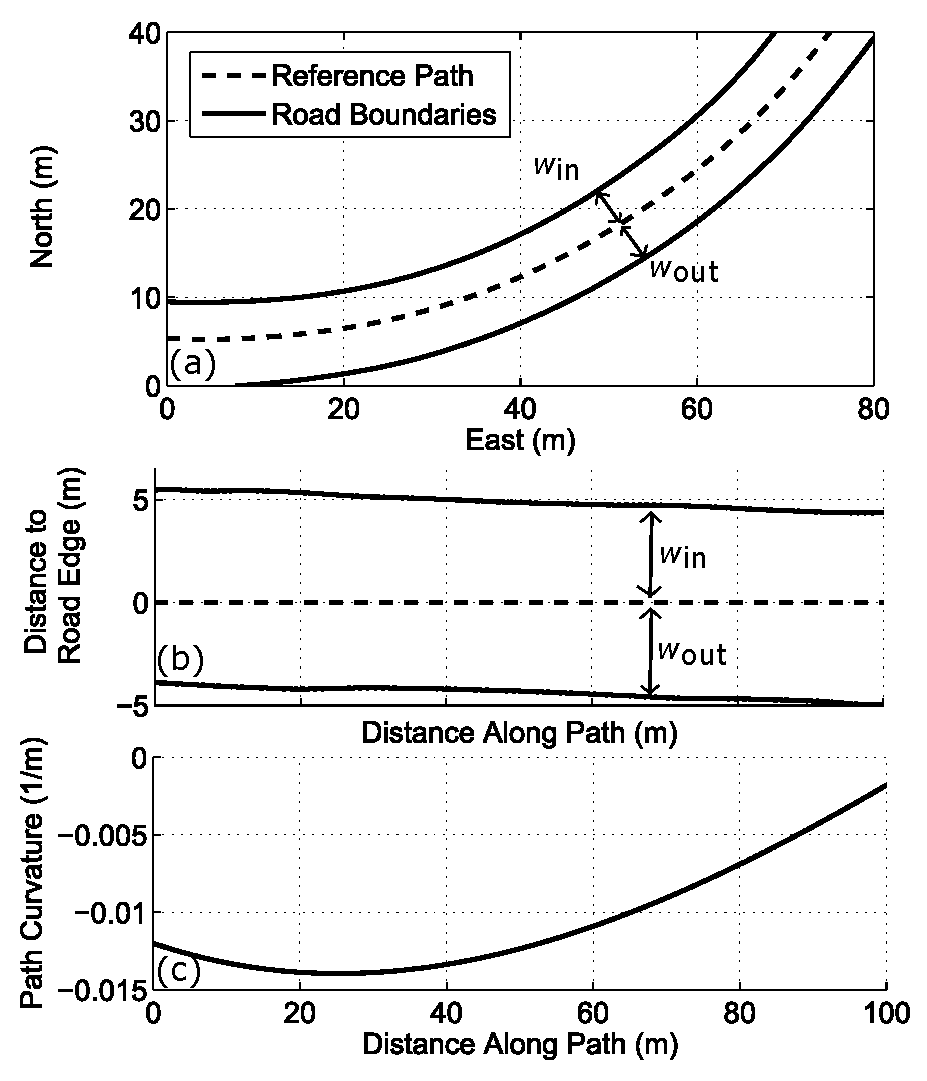
\includegraphics[width=.85\fullwidth]{worldInfo.eps}
\caption[View of sample reference path and road boundaries]{(a) View of a sample reference path and road boundaries, plotted in the East-North Cartesian frame (b) Lateral distance from path to inside road edge (positive) and outside road edge (negative) as a function
of distance along path. (c) Curvature as a function of distance along path.}
\label{fig:worldInfo}
\end{figure}

\section{Velocity Profile Generation Given Fixed \newline Reference Path}
\label{sec:VP}

Given a fixed reference path described by $s$ and $\kappa$, the first algorithm step is to find the 
minimum-time speed profile the vehicle can achieve
without exceeding the available friction. 
While finding the minimum-time speed profile for a fixed path was recently solved as a convex problem by Lipp and Boyd \cite{lipp}, the
 algorithm presented in this chapter directly uses the ``three-pass" approach described by 
Subosits and Gerdes \cite{subosits}, and originally inspired by work from Velenis and Tsiotras \cite{velenis}
and Griffiths \cite{griffiths}. 
Given the lumped front and rear tires from the bicycle model, the available longitudinal
 and lateral forces $F_\mathrm{x}$ and $F_\mathrm{y}$ at each wheel are constrained by the friction circle: 
\begin{subequations}
\label{eq:tireforce}
\begin{align}
	F^2_\mathrm{xf} + F_\mathrm{yf}^2 &\leq (\mu F_\mathrm{zf})^2\\
	F^2_\mathrm{xr} + F_\mathrm{yr}^2 &\leq (\mu F_\mathrm{zr})^2
\end{align}
\end{subequations}
where $\mu$ is the tire-road friction coefficient and $F_\mathrm{z}$ is the available normal force. The first pass of the speed profile generation finds the maximum permissible
 vehicle speed given zero longitudinal force. For the simplified case where weight transfer and topography effects are neglected, this is given by:
\begin{equation}
\label{eq:steadystate}
	U_x(s) = \sqrt{\frac{\mu g}{|\kappa(s)|}}
\end{equation}
where the result in (\ref{eq:steadystate}) is  obtained by setting $F_\mathrm{yf} = \frac{mb}{a+b}U_x^2\kappa$ and $F_\mathrm{zf} = \frac{mgb}{a+b}$.
 The results of this first pass for the sample curvature profile in Fig.~\ref{fig:VPgen}(a) are shown in Fig.~\ref{fig:VPgen}(b).
 The next step is a forward 
integration step, where the velocity of a given point is determined by the velocity of the previous point and the available longitudinal force $F_{x,\mathrm{max}}$ for acceleration.
This available longitudinal force is calculated in \cite{subosits} by accounting for the vehicle engine force limit and the lateral force demand on all tires due to the road curvature:
\begin{equation}
\label{eq:forwardint}
	U_x(s+\Delta s) =\sqrt{U^2_x(s)+\mathrm{2}\frac{F_{x,\mathrm{accel,max}}}{m}\Delta s}
\end{equation}
A key point of the forward integration step is that at every point, the value of $U_x(s)$ is compared to the corresponding value from (\ref{eq:steadystate}), and
the minimum value is taken. The result is shown graphically in Fig.~\ref{fig:VPgen}(c). Finally, the backward integration step occurs, where the available
longitudinal force for deceleration is again constrained by the lateral force demand on all tires:
\begin{equation}
\label{eq:backwardsint}
	U_x(s-\Delta s) = \sqrt{U^2_x(s)-\mathrm{2}\frac{F_{x,\mathrm{decel,max}}}{m}\Delta s}
\end{equation}
The value of $U_x(s)$ is then compared to the corresponding value from (\ref{eq:forwardint}) for each point along the path, and the minimum
value is chosen, resulting in the final velocity profile shown by the solid line in Fig.~\ref{fig:VPgen}(d). While treatment of three-dimensional road 
effects are not described in this chapter, the method described in \cite{subosits} and
used for the experimental data collection determines the normal and lateral tire forces $F_\mathrm{z}$ and $F_\mathrm{y}$ at each point along the path 
by accounting for weight transfer and bank/grade of the road surface. 

 \begin{figure}
\centering
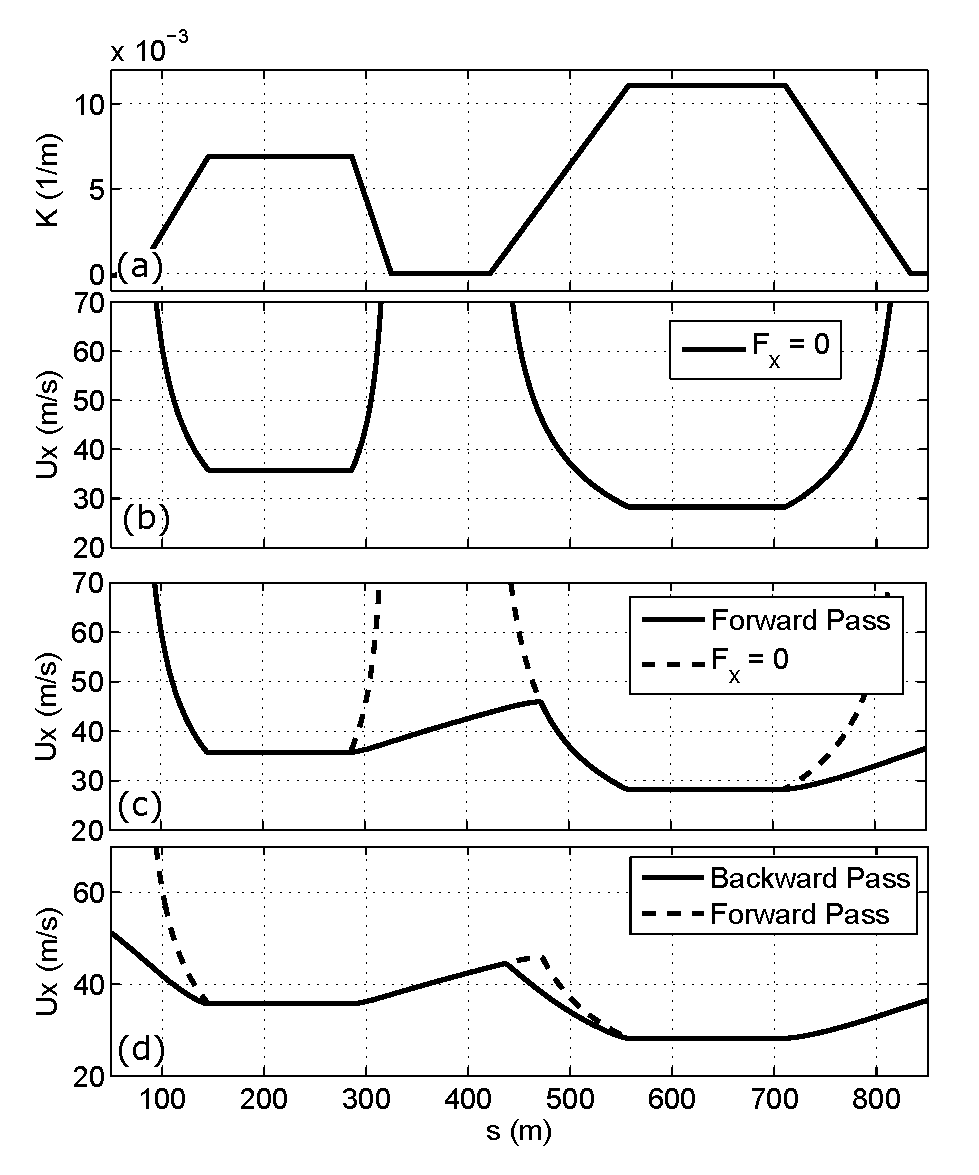
\includegraphics[width=\fullwidth]{vpgen.eps}
\caption[Velocity profile generation illustration]{(a) Sample curvature profile. (b) Velocity profile given zero longitudinal force. (c) Velocity profile after forward pass. (d) Final velocity profile after backward pass. }
\label{fig:VPgen}
\end{figure}

\section{Updating Path Given Fixed Velocity Profile}
\label{sec:UPDATE}
\subsection{Overall Approach and Minimum Curvature Heuristic}
The second step of the trajectory generation algorithm takes the original reference path $\kappa(s)$ and corresponding velocity profile $U_x(s)$
as inputs, and modifies the reference path to obtain a new, ideally faster, racing line. Sharp \cite{sharp} suggests a general approach for modifying 
an initial path to obtain a faster lap time by taking the original path and velocity profile and incrementing the speed uniformly
by a small, constant ``learning rate." An optimization problem is then solved to find a new reference path and control inputs that allow the vehicle to
drive at the higher speeds without driving off the road. If a crash is detected, the speed inputs are locally reduced around the crash site and the process is repeated.

However, one challenge with this approach is that it can take several hundred iterations of locally modifying the vehicle speed profile, detecting crashes, and 
 modifying the reference path to converge to a fast lap time. An alternative approach is to modify the reference path in one step by solving a single 
 optimization problem. The lap time $t$ for a given racing line is provided by the following equation: 
 
 \begin{equation}
t = \int_0^l\frac{ds}{U_x(s)}
\label{integrateEq}
\end{equation}
 
 Equation (\ref{integrateEq}) implies that minimizing the vehicle lap time requires simultaneously minimizing the total path length $l$ while maximizing
 the vehicle's longitudinal velocity $U_x$. These are typically competing objectives, as lower curvature (i.e. higher radius) paths can result in longer path lengths but higher
 vehicle speeds when the lateral force capability of the tires is reached, as shown in (\ref{eq:steadystate}). Since (\ref{integrateEq}) is a nonconvex cost function in the
 optimization variables, time-intensive nonlinear programming is required to manage this curvature/distance trade-off and explicitly minimize the lap time. 
 
 The proposed approach is therefore to simplify the cost function by only minimizing the norm of the vehicle's driven curvature
 $\kappa(s)$ at each path modification step. Path curvature can be easily formulated as a convex function with respect to the vehicle state vector $x$, 
 enabling the path modification step to be easily solved by leveraging the computational speed of convex optimization. 
 
 However, minimizing curvature is not the same as minimizing lap time and provides
 no guarantee of finding the time-optimal solution. The proposed cost function relies on the hypothesis that a path with minimum curvature is a good approximation for
 the minimum-time racing line. Lowering the curvature of the racing line is more important than minimizing
 path length for most race courses, as the relatively narrow track width provides limited room to shorten the overall path length. Simulated and experimental results
 in \S \ref{sec:IMPLEMENT} and  \S \ref{sec:EXP} will validate this hypothesis by showing similar lap time performance when compared to
 a gradient descent method that directly minimizes lap time. However, a particular section of the race track where the minimum curvature
 solution shows poor performance will be discussed as well, and improved upon in \S \ref{sec:ADDMINDIST}. 

\subsection{Convex Problem Formulation}

Formulating the path update step as a convex optimization problem requires an affine, discretized form of the
bicycle model presented earlier. The equations of motion in (\ref{eq:bm}) are already linearized, but
 the front and rear lateral tire forces become saturated as the vehicle drives near the limits of tire adhesion. 
The well-known brush tire model \cite{Pacejka2012}, also presented in Chapter 2, captures the effect of tire saturation:
\begin{eqnarray}
\label{eq:fiala}
	F_\mathrm{y\diamond}&=&\begin{cases} -C_{\diamond}\tan\alpha_\diamond + \frac{C_\diamond^2}{3\mu F_\mathrm{z\diamond}} |\tan\alpha_\diamond| \tan\alpha_\diamond \\ \hspace{10mm}- \frac{C_\diamond^3}{27\mu^2F_\mathrm{z\diamond}^2}\tan^3\alpha_\diamond,
\hspace{8mm}  |\alpha_\diamond| < \arctan{\left(\frac{3\mu F_\mathrm{z\diamond}}{C_\diamond}\right)} \\ \\ -\mu F_\mathrm{z\diamond}\text{sgn} \ \alpha_\diamond, \hspace{36mm} \mathrm{otherwise} \end{cases}
\end{eqnarray}
where the symbol $\diamond \in [\mathrm{f},\mathrm{r}]$ denotes the lumped front or rear tire, and $C_\diamond$ is the corresponding tire cornering stiffness. 

\newpage
The linearized tire slip angles $\alpha_\mathrm{f}$ and $\alpha_\mathrm{r}$ are functions of the vehicle lateral states and the steer angle
input, $\delta$:
\begin{subequations}
\begin{align}
	\alpha_\mathrm{f} &= \beta + \frac{ar}{U_x} - \delta\\
	\alpha_\mathrm{r} &= \beta - \frac{br}{U_x}
\end{align}
\end{subequations}
The brush tire model in (\ref{eq:fiala}) can be linearized at every point along the reference path assuming steady state cornering conditions:
\begin{subequations}
\begin{align}
	F_\mathrm{y\diamond} &= \tilde{F}_\mathrm{y\diamond} - \tilde{C}_\diamond(\alpha_\diamond - \tilde{\alpha}_\diamond) \\
	\tilde{F}_\mathrm{y\diamond} &= \frac{F_\mathrm{z\diamond}}{g} U_x^2\kappa
\label{eqn:ftil}
\end{align}
\end{subequations}
with parameters $\tilde{F}_\mathrm{y}$, $\tilde{\alpha}$ and $\tilde{C}$ shown in Fig.~\ref{fig:fiala}. 

\begin{figure}[h]
\centering
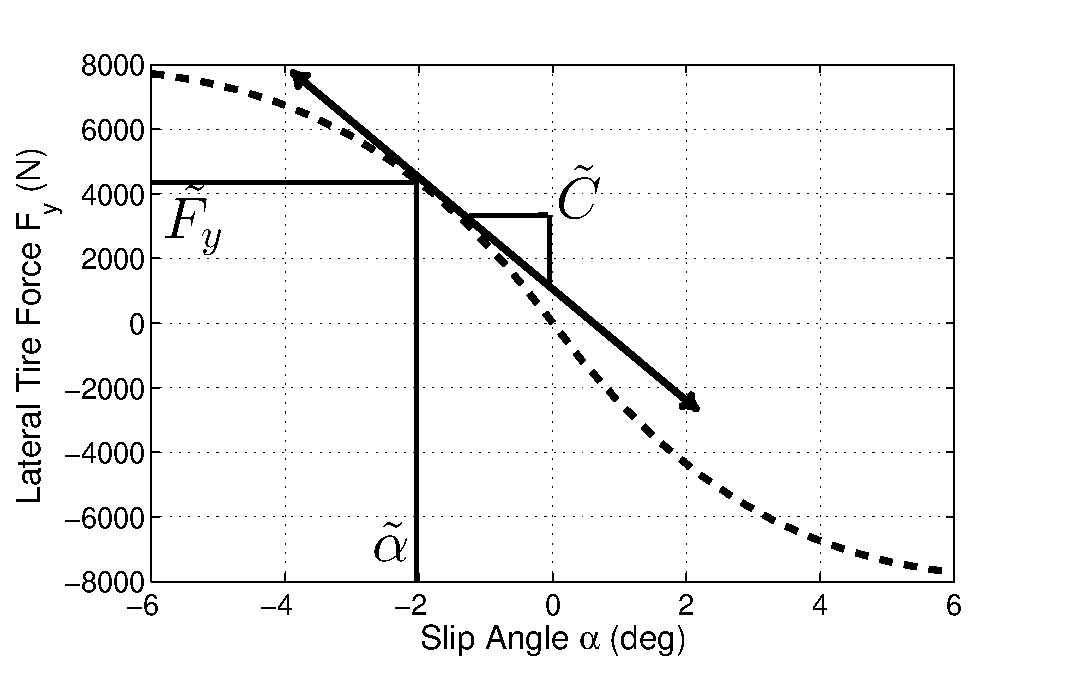
\includegraphics[width=.9\fullwidth]{fiala.eps}
\caption{Nonlinear tire force curve given by Fiala model, along with affine tire model linearized at $\alpha = \tilde{\alpha}$. }
\label{fig:fiala}
\end{figure}

The affine, continuous bicycle model with
steering input $\delta$ is then written in state-space form as:
\begin{subequations}
\label{eq:cts}
\begin{align}
	\dot{x}(t) &= A(t) x + B(t)\delta + d(t)\\
	 x &= [e \hspace{2mm} \Delta\Psi \hspace{2mm} r \hspace{2mm} \beta \hspace{2mm} \Psi]^T
\end{align}
\end{subequations}
where we have added a fifth state, vehicle heading angle $\Psi$, defined as the time integral of yaw rate $r$.
 This makes explicit computation of the minimum curvature path simpler. The state matrices $A(t)$, $B(t)$, and affine term $d(t)$ 
 are given by:
\begin{align}
A(t)  &= \left[\begin{matrix}
  0 & U_x(t) & 0 & U_x(t) & 0\\ 
  0 & 0 & 1 & 0 & 0 \\ 
  0 & 0  & \frac{-a^2\tilde{C}_\mathrm{f}(t)-b^2\tilde{C}_\mathrm{r}(t)}{U_x(t)I_\mathrm{z}} & \frac{b\tilde{C}_\mathrm{r}(t) - a\tilde{C}_\mathrm{f}(t)}{I_\mathrm{z}} & 0 \\
  0 & 0  & \frac{b\tilde{C}_\mathrm{r}(t)-a\tilde{C}_\mathrm{f}(t)}{mU_x^2(t)}-1 & \frac{-\tilde{C}_\mathrm{f}(t) - \tilde{C}_\mathrm{r}(t)}{mU_x(t)} & 0 \\
  0 & 0 & 1 & 0 & 0
 \end{matrix}\right] \\
B(t) &=[0 \hspace{2 mm} 0 \hspace{3 mm} \frac{a \tilde{C}_\mathrm{f}(t)}{I_\mathrm{z}} \hspace{3 mm}  \frac{\tilde{C}_\mathrm{f}(t)}{mU_x(t)} \hspace{3mm} 0]^T \\
d(t) &= \left[\begin{matrix} 0 \\
               -\kappa(t) U_x(t) \\ 
			    \frac{a\tilde{C}_\mathrm{f}(t)\tilde{\alpha}_\mathrm{f}(t) - b\tilde{C}_\mathrm{r}(t)\tilde{\alpha}_\mathrm{r}(t) + a\tilde{F}_\mathrm{yf}(t) - b\tilde{F}_\mathrm{yr}(t)}{I_z} \\
				\frac{\tilde{C}_\mathrm{f}(t)\tilde{\alpha}_\mathrm{f}(t) + \tilde{C}_\mathrm{r}(t)\tilde{\alpha}_\mathrm{r}(t) + \tilde{F}_\mathrm{yf}(t) + \tilde{F}_\mathrm{yr}(t)}{mU_x(t)}\\
				0
				\end{matrix}\right]
\end{align}

With the nonlinear model approximated as an affine, time-varying model, updating the path is accomplished by solving the following
 convex optimization problem:

\begin{subequations}
\label{eq:OPT}
\begin{alignat}{3}
\underset{\delta, \hspace{.5mm} x}{\text{minimize}} \quad & \sum_{k} \left(\frac{\Psi_k - \Psi_{k-1}}{s_k - s_{k-1}}\right)^2 + \lambda(\delta_k - \delta_{k-1})^2 & \quad  \label{eq:obj}\\
{\text{subject to}} \quad & \rlap{$ x_{k+1}= A_k x_k + B_k \delta_k + d_k$} \label{jenny}\\
& \rlap{$w^\mathrm{out}_k \leq e_k \leq w^\mathrm{in}_k $} \label{bobby}\\
& \rlap{$x_1 = x_T$\label{keylani}}
\end{alignat}
\end{subequations}
where $k = 1 \dots T$ is the discretized time index, and $A_k$, $B_k$, and $d_k$ are discretized versions of the continuous state-space
equations in (\ref{eq:cts}). The objective function (\ref{eq:obj}) minimizes the curvature norm of the path driven by the vehicle, as path curvature is
the derivative of the vehicle heading angle with respect to distance along the path $s$ (\ref{eq:balls}). To maintain convexity of the objective
function, the term ${s_k - s_{k-1}}$ is a constant rather than a variable, and is updated for the next iteration after the optimization has been completed (see \S \ref{sec:IMPLEMENT}).
Additionally, there is a regularization term with weight $\lambda$ added in the cost function to ensure a smooth steering profile for experimental 
implementation. 

\begin{figure}[h]
\centering
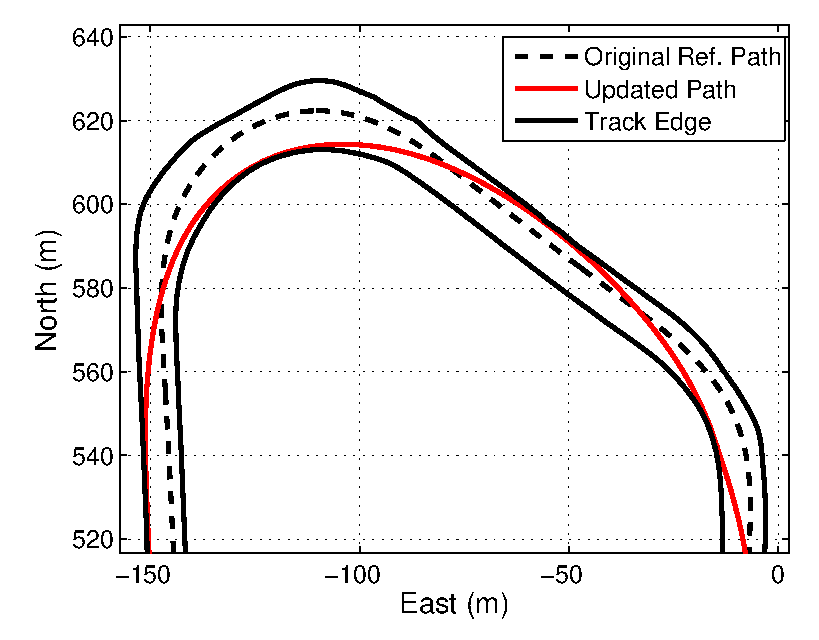
\includegraphics[width=.7\fullwidth]{updatedpath.eps}
\caption{Path update for an example turn.}
\label{fig:hairpin}
\end{figure}


The equality constraint (\ref{jenny}) ensures the vehicle follows the affine lateral dynamics. The inequality
 constraint (\ref{bobby}) allows the vehicle to deviate laterally from the reference path to find a new path with lower curvature, but
 only up to the road edges. Finally, the equality constraint (\ref{keylani}) is required for complete racing circuits to ensure the generated
 racing line is a continuous loop. The results of running the optimization 
 are shown for an example turn in Fig.~\ref{fig:hairpin}. The reference path starts out at the road centerline, and the optimization finds 
 a modified path that uses all the available width of the road to lower the path curvature. Note that the available road widths $w_\mathrm{in}$ and
 $w_\mathrm{out}$ have an offset built in to account for the width of the vehicle. 

 
\section{Algorithm Implementation and Simulated \newline Results}
\label{sec:IMPLEMENT}
\subsection{Algorithm Implementation}
The final algorithm for iteratively
generating a vehicle racing trajectory is described in Fig.~\ref{algorithmDesc}. 
The input to the algorithm is any initial path through the racing circuit, 
parameterized in terms of distance along the path $s$, path curvature $\kappa(s)$, and the lane edge distances $w_\mathrm{in}(s)$ and 
$w_\mathrm{out}(s)$ from Fig.~\ref{fig:worldInfo}.
 \begin{figure}
\begin{algorithmic}[1]
\Procedure{GenerateTrajectory}{$s^0, \kappa^0, w_\mathrm{in}^0, w_\mathrm{out}^0$}
\State $\mathrm{path}\gets (s^0, \kappa^0, w_\mathrm{in}^0, w_\mathrm{out}^0)$
\While{$\Delta t^\star > \epsilon$}
\State $U_x \gets \mathrm{calculateSpeedProfile(path)}$
\State $\mathrm{path} \gets \mathrm{minimizeCurvature}(U_x, \mathrm{path})$
\State $t^\star \gets \mathrm{calculateLapTime}(U_x,\mathrm{path})$
\EndWhile
\State \textbf{return} $\mathrm{path},U_x$
\EndProcedure
\end{algorithmic}
\caption[Iterative algorithm for fast generation of vehicle trajectories.]{Iterative algorithm for fast generation of vehicle trajectories. Each iteration consists of a sequential two-step approach where
the velocity profile is generated given a fixed path and then the path is updated based on the solution from a convex optimization problem.}\label{algorithmDesc}
\end{figure}

 Given the initial path, the minimum-time speed profile $U_x(s)$ is calculated using the
approach from \S \ref{sec:VP}. Next, the path is modified by solving the minimum curvature
 convex optimization problem (\ref{eq:OPT}). 
 

 
The optimization only solves explicitly for the steering input $\delta^\star$ and resulting vehicle lateral states $x^\star$ at every 
time step. Included within $x^\star$  is the optimal vehicle heading $\Psi^\star$ and lateral deviation $e^\star$ from the initial path. To obtain 
the new path in terms of $s$ and $\kappa$, the East-North coordinates ($E_k$, $N_k$) of the updated vehicle path are updated as follows:
	
\begin{subequations}
\begin{align}
	E_k &\gets E_k - e^\star_k\cos(\Psi_{\mathrm{r},k})\\
	N_k &\gets N_k - e^\star_k\sin(\Psi_{\mathrm{r},k})
\end{align}
\end{subequations}
where $\Psi_\mathrm{r}$ is the path heading angle of the original path. Next, the new path is given by the following numerical approximation:
 \begin{subequations}
 \label{eq:pupdate}
\begin{align}
	s_k &= s_{k-1} + \sqrt{(E_k - E_{k-1})^2 + (N_k - N_{k-1})^2}\\ 
	\kappa_k &= \frac{\Psi^\star_k - \Psi^\star_{k-1}}{s_k - s_{k-1}}
\end{align}
\end{subequations}
 Notice that (\ref{eq:pupdate}) accounts for the change in the total path length that occurs when the vehicle deviates from the original path.
 In addition to $s$ and $\kappa$, the lateral distances to the track edges $w_\mathrm{in}$ and $w_\mathrm{out}$ are different for the new path
 as well, and are recomputed using the Cartesian coordinates for
the inner and outer track edges and ($E_k$, $N_k$). The two-step procedure is iterated until the improvement in lap time $\Delta t^\star$ over the prior iteration is less than a small positive 
constant $\epsilon$.


\begin{table}
\label{tb:optprm}
\begin{center}
\small
\caption{Optimization Parameters}\label{tb:optprm}
\begin{tabular}{lccc}
Parameter & Symbol & Value & Units \\\hline
Regularization Parameter & $\lambda$ & 1 & $\mathrm{1/m}^2$\\
Stop Criterion           & $\epsilon $ & 0.1 & s \\
Vehicle mass & $m$ & 1500 & kg \\
Yaw Inertia & $I_z$ & 2250 & $\mathrm{kg \cdot m}^2$\\
Front axle to CG & $a$ & 1.04 & m\\
Rear axle to CG & $b$ & 1.42 & m\\
Front cornering stiffness & $\mathrm{C}_\mathrm{f}$ & 160 & $\mathrm{kN \cdot rad}^{-1}$ \\
Rear cornering stiffness & $\mathrm{C}_\mathrm{r}$ & 180 & $\mathrm{kN \cdot rad}^{-1}$ \\
Friction Coefficient     & $\mu $                  &  0.95 & $\mathrm{-} $ \\
Path Discretization      & $\Delta s$              & 2.75 & $m$\\
Optimization Time Steps  & $T       $              & 1843 & -  \\
Max Engine Force         & -                       & 3750 & N\\\hline
\end{tabular}
\end{center}
\end{table}

\subsection{Algorithm Validation}
The proposed algorithm is tested by analyzing the lap time performance on
 the same racing circuit and Audi TTS experimental test vehicle described in
Chapter 2. The vehicle parameters 
used for the lap time optimization are shown along with the optimization parameters in Table \ref{tb:optprm}.
 The initial path is obtained by collecting GPS data of the inner and outer track edges and estimating the ($s, \kappa, w_\mathrm{in}, w_\mathrm{out}$)
 parametrization of the track centerline via a separate curvature estimation subproblem similar to the one proposed in \cite{perantoni}.
 The algorithm is implemented in MATLAB, with the minimum curvature optimization problem (\ref{eq:OPT}) solved using the CVX software package \cite{boydcvx} and
 the speed profile generation problem solved using a library from Subosits and Gerdes \cite{subosits}.

 \begin{figure}
\centering
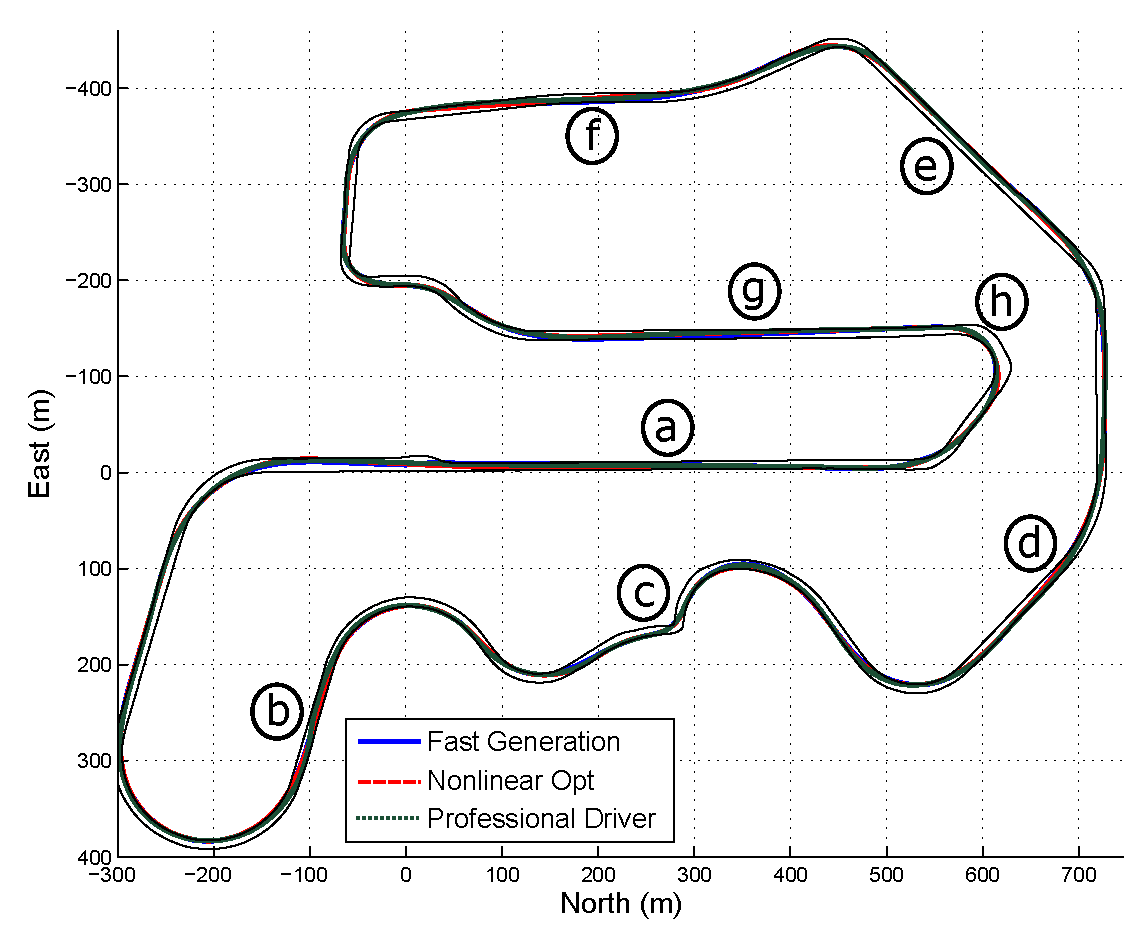
\includegraphics[width=\fullwidth]{racinglines.eps}
\caption[Overhead view of Thunderhill Raceway park along with generated path from algorithm.]{Overhead view of Thunderhill Raceway park along with generated path from algorithm. Car drives in alphabetical direction around the closed circuit. Labeled regions a-h are locations of discrepancies between the 
two-step algorithm solution and comparison solutions.}
\label{racingLines}
\end{figure}
\subsection{Comparison with Other Methods}
The generated racing path after five iterations is shown in
Fig.~\ref{racingLines}. To validate the proposed algorithm, the racing line is compared with results from a nonlinear gradient descent algorithm implemented by 
Theodosis and Gerdes \cite{theodosis} and an experimental trajectory recorded from a professional racecar driver in the experimental testbed vehicle.
 While time-intensive to compute, experimental lap times from the gradient descent trajectory are within one second of
lap times from professional racecar drivers. 

To better visualize the differences between all three racing lines, Fig.~\ref{fig:pathDeviation} shows the lateral deviation from the track centerline as a function of distance along the centerline 
for all three trajectories. The left and right track boundaries $w_\mathrm{in}$ and $w_\mathrm{out}$ are plotted as well. The two-step iterative algorithm provides a 
racing line that is qualitatively similar to the gradient descent and human driver racing lines. In particular, all three
solutions succeed at utilizing the available track width whenever possible, and strike similar apex points for each
of the circuit's 15 corners. 

\begin{figure}
\centering
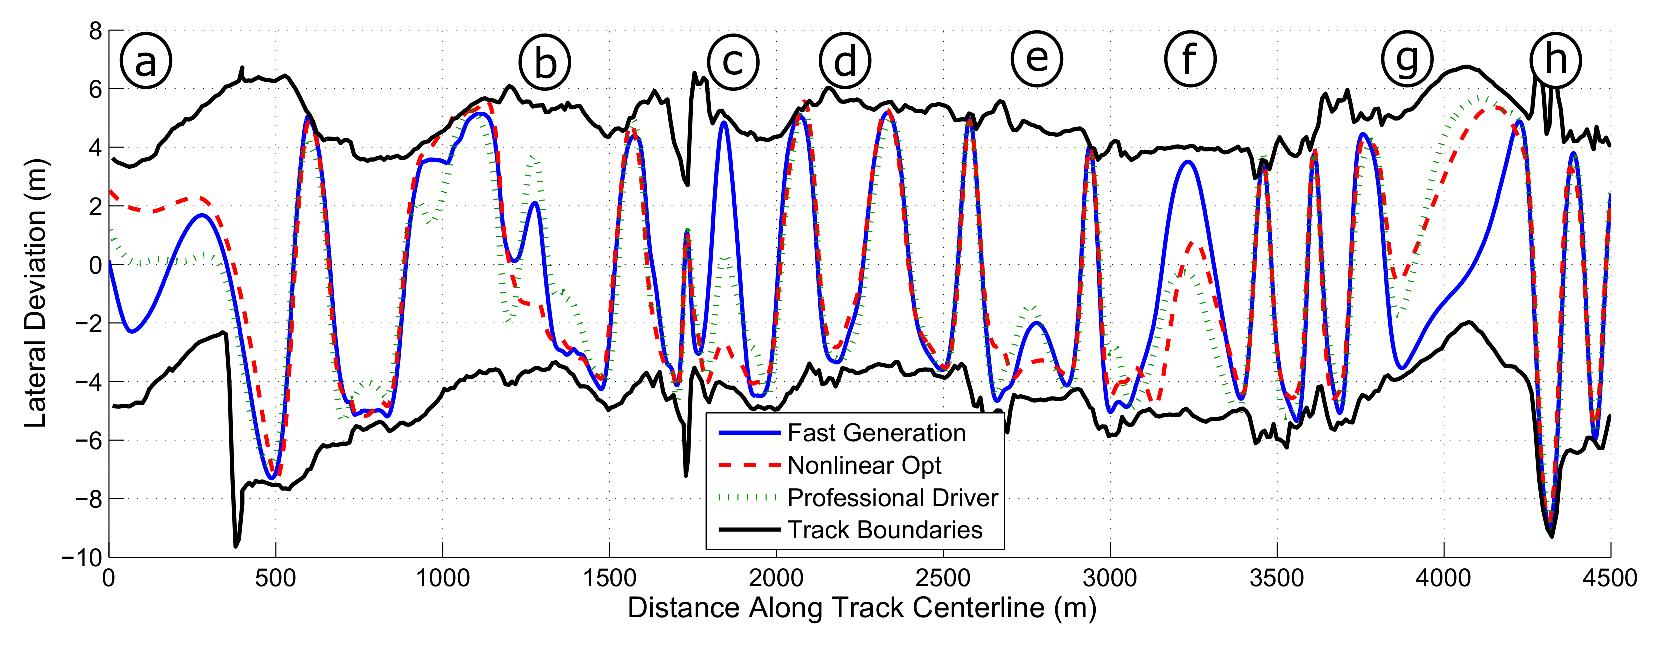
\includegraphics[width=\fullwidth]{deviationFromCenterline.eps}
\caption[Lateral path deviation of racing line from track centerline as a function of distance along the centerline.]{Lateral path deviation of racing line from track centerline as a function of distance along the centerline. Note that upper and lower bounds on $e$ are not always symmetric
due to the initial centerline being a smooth approximation. Results
are compared with racing line from a nonlinear gradient descent algorithm and experimental data recorded from a professional racecar driver.}
\label{fig:pathDeviation}
\end{figure}	

However, there are several locations on the track where there is a significant discrepancy (on the order of several meters) between the two-step algorithm's trajectory and the 
other comparison trajectories. These locations of interest are labeled \circled{a} through \circled{h} in Fig.~\ref{racingLines}.
Note that sections \circled{a}, \circled{e}, \circled{f}, and \circled{g} all occur on large, relatively straight portions of the racing circuit.
In these straight sections, the path curvature is relatively low and differences in lateral deviation from the track centerline have a relatively small
effect on the lap time performance.   

Of more significant interest are the sections labeled \circled{b}, \circled{c}, \circled{d}, and \circled{h}, which all occur at turning regions of the track.
These regions are plotted in Fig.~\ref{compositeFig1} and Fig.~\ref{compositeFig2} for zoomed-in portions of the race track. While it is difficult to analyze a single turn
of the track in isolation, discrepancies can arise between the two-step fast generation method and the gradient descent as the latter method trades off 
between minimizing curvature and distance traveled. As a result, the gradient descent method finds
 regions where it may be beneficial to use less of the available road width in order to reduce the total distance
traveled. In region \circled{b}, for example, the fast generation algorithm exits the turn and gradually approaches the left side in order to create space for the
upcoming right-handed corner. The nonlinear optimization, however, chooses a racing line that stays toward the right side of the track. 
In this case, the behavior of the human driver more closely matches that of the two-step fast generation algorithm.

 \begin{figure}[tb]
\centering
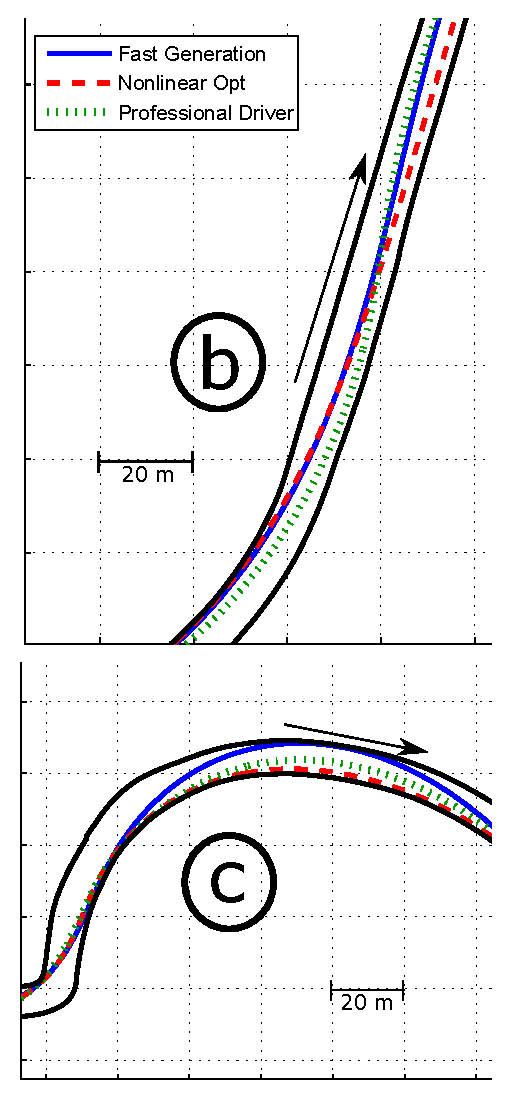
\includegraphics[width=\fullwidth]{composite1.eps}
\caption[Racing lines from the two-step fast generation approach, nonlinear gradient descent algorithm, and experimental data taken
from professional driver.]{Racing lines from the two-step fast generation approach, nonlinear gradient descent algorithm, and experimental data taken
from professional driver. Car drives in direction of labeled arrow.}
\label{compositeFig1}
\end{figure}

 \begin{figure}[tb]
\centering
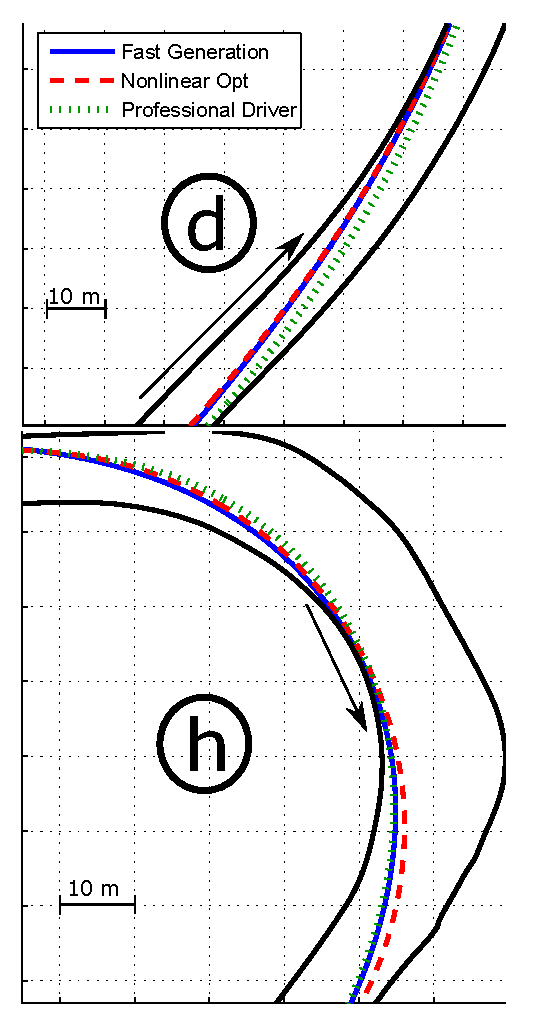
\includegraphics[width=\fullwidth]{composite2.eps}
\caption[Racing lines from the two-step fast generation approach, nonlinear gradient descent algorithm, and experimental data taken
from professional driver.]{Racing lines from the two-step fast generation approach, nonlinear gradient descent algorithm, and experimental data taken
from professional driver. Car drives in direction of labeled arrow.}
\label{compositeFig2}
\end{figure}	

 The human driver also drives closer to the 
fast generation solution in \circled{h}, while the gradient descent algorithm picks a path that exits the corner with a larger radius. In section \circled{c}, the gradient descent
algorithm again prefers a shorter racing line that remains close the the inside edge of the track, while the two-step algorithm drives all the way
to the outside edge while making the right-handed turn. Interestingly, the human driver stays closer to the middle of the road, but more closely
follows the behavior of the gradient descent algorithm. There are also regions of the track where the computational algorithms pick a similar path that 
differs from the human driver, such as region \circled{d}.
 
\subsection{Lap Time Convergence and Predicted Lap Time}
Fig.~\ref{lapTimes} shows the predicted lap time for each iteration of the fast generation algorithm, with step 0 corresponding
to the initial race track centerline. The lap time was estimated after each iteration by numerically simulating a vehicle 
 following the desired path and velocity profile using a closed-loop controller. The equations of motion for the simulation
were the nonlinear versions of (\ref{eq:bm}) with tire forces given by
the brush tire model in (\ref{eq:fiala}). 

\begin{figure}
\centering
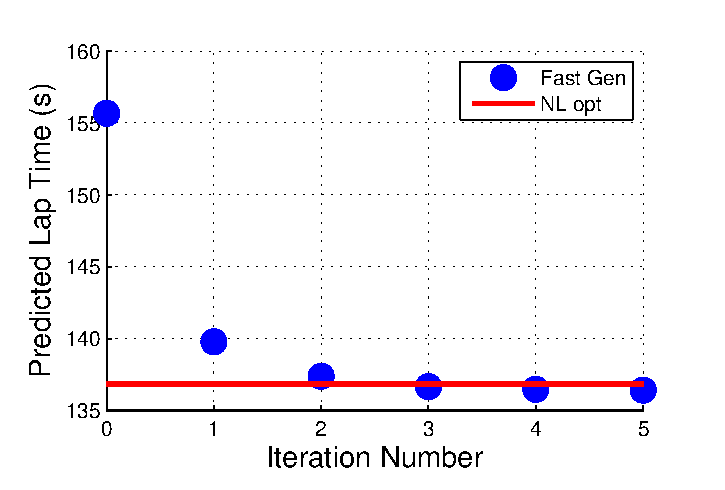
\includegraphics[width=.8\fullwidth]{laptimes.eps}
\caption[Lap time as a function of iteration for the two-step fast trajectory generation method.]{Lap time as a function of iteration number for the two-step fast trajectory generation method. Final lap time is comparable
to that achieved with the nonlinear gradient descent approach. Iteration zero corresponds to the lap time for driving the track centerline.}
\label{lapTimes}
\end{figure}

Fig.~\ref{lapTimes} shows that the predicted lap time converges monotonically over four or five iterations, with significant 
improvements over the centerline trajectory occuring over the first two iterations. The predicted minimum lap time of 136.4 seconds
is similar to the predicted lap time of 136.7 seconds from the nonlinear gradient descent, 
although in reality, the experimental lap time will depend significantly on unmodeled effects such 
as powertrain dynamics.  

The final curvature and velocity profile for the two-step  method is compared with the equivalent profiles for the gradient
descent algorithm in Fig.~\ref{fig:simData}. Notice that the piecewise linear $\kappa(s)$ for the gradient descent
 is due to the clothoid constraint imposed by \cite{theodosis} for ease of autonomous path following. 

 \begin{figure}[tb]
\centering
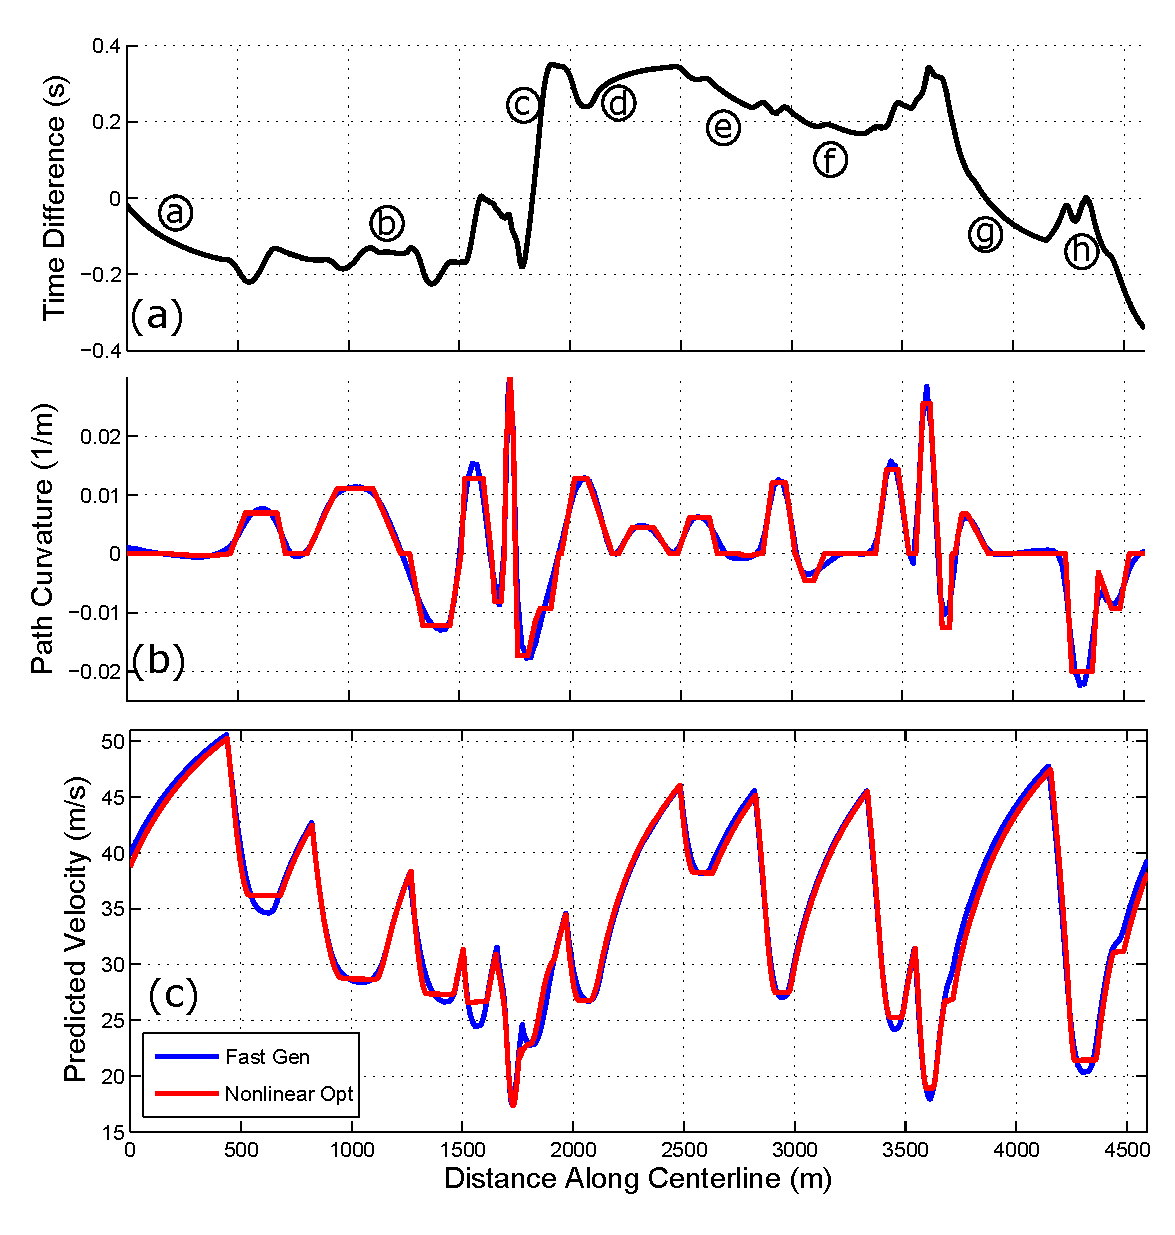
\includegraphics[width=\fullwidth]{simData.eps}
\caption[Simulation results of fast generation algorithm]{(a) Predicted time difference between a car driving both trajectories, with a negative
value corresponding the two-step algorithm being ahead. (b) Curvature profile $\kappa(s)$ plotted vs. distance along the path $s$.
 (c) Velocity profile $U_x(s)$ plotted 
vs. distance along the path $s$ for the two-step method and nonlinear gradient descent method.}
\label{fig:simData}
\end{figure} 
\newpage
In general, the curvature and velocity profiles are very similar, although the fast generation algorithm results in a velocity profile
with slightly lower cornering speeds but slightly higher top speeds.
The predicted time difference between a car driving both trajectories 
is shown in Fig.~\ref{fig:simData}(a), with a negative
value corresponding the two-step algorithm being ahead. 

Notice that in region \circled{c}, the trajectory from the two-step algorithm performs
poorly, losing almost a half second of time to the nonlinear optimization over just 150 meters. Referring back to Fig.~\ref{compositeFig1}, 
region \circled{c} is a sweeping right-hand turn that comes after a very tight left-hand turn on the track, and both the human driver
and nonlinear optimization prefer to take a shorter path and stay closer to the inside edge of the track. While this results in a higher
curvature for the first turn, the shorter path on the second turn creates a net time advantage. As a result, the gradient descent optimization from Theodosis
and Gerdes \cite{theodosis} retains an overall time advantage from this turn
on until losing ground in section \circled{g}, where the two-step method catches up and ultimately completes the lap with a 0.3 second time advantage. 
The difference between the two techniques suggests that neither is a globally optimal solution, since the minimum curvature heuristic proposed here and the restriction
to clothoid segments in \cite{theodosis} are not mutually exclusive and benefits of both could be combined to further improve the lap time. 

\section{Experimental Setup} 
\label{sec:EXP}
While the two-step algorithm works well in simulation, the most critical validation step is to have an
autonomous race car drive the generated trajectory. This was accomplished by 
collecting experimental data on the Audi TTS.  

The experimental controller setup is shown in Fig.~\ref{fig:expSetupC3} 
and is very similar to that presented in Chapter 2. The main two differences in the controller are highlighted
in red. Instead of using the piecewise linear clothoid  curvature profile from Theodosis and Gerdes \cite{theodosis}, the trajectory
from the presented algorithm is applied. This trajectory is 
represented mathematically as an array of discrete points. This point cloud is relatively
dense, with each point spaced about 25 cm apart over the entire path.

Since the trajectory is now a set of discrete points rather than a piecewise linear $\kappa(s)$ function, the localization algorithm cannot rely on Newton-Raphson gradient descent. Instead, a
simple search algorithm iterates through the point cloud and finds the closest two points to the vehicle's center of
gravity. Bisection is applied to the find the closest distance between the vehicle and the line connecting these
two points on the point cloud. To save the expense of searching the entire point cloud on every iteration, 
the localization starts the search algorithm where the last iteration terminated and searches only a small region
of the entire map. 

\begin{figure}[tb]
\centering
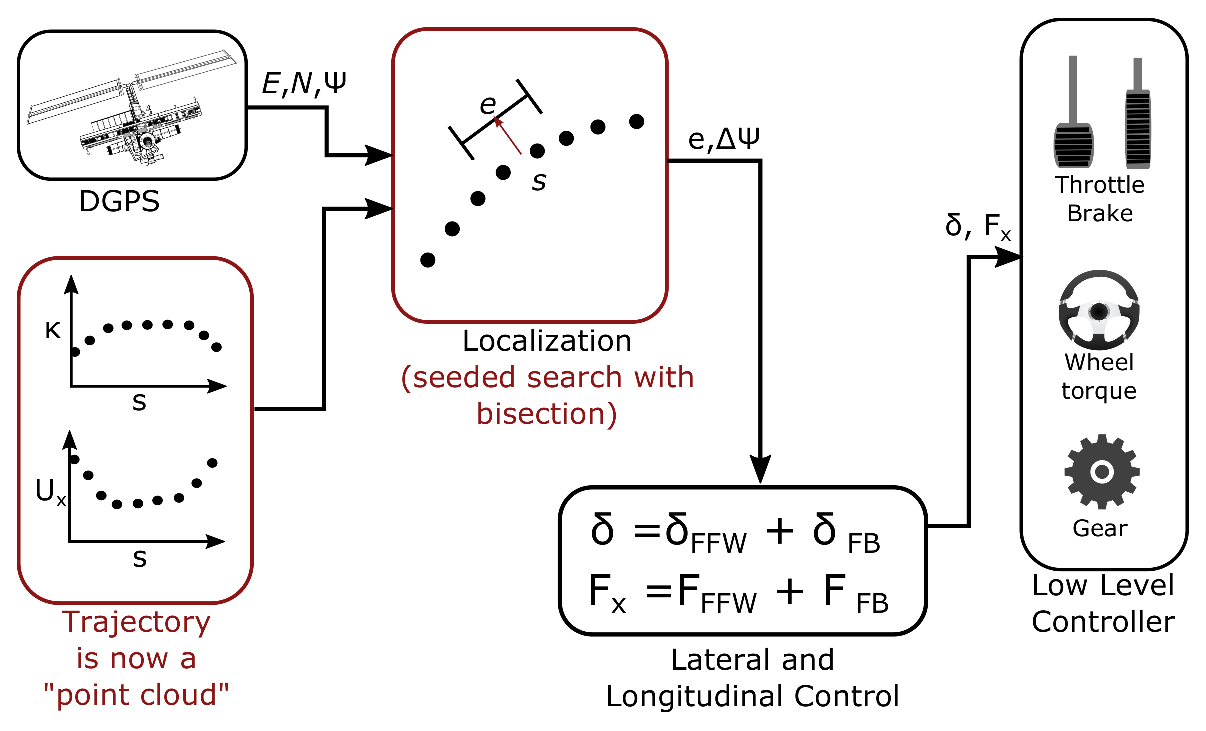
\includegraphics[width=\fullwidth]{expSetupC3.eps}
\caption{Diagram of controller setup.}
\label{fig:expSetupC3}
\end{figure}

\section{Experimental Results}
\label{sec:ch3ExpRes}

The resulting experimental lap time for the iterative two-step algorithm was 138.6 seconds, about 0.6 seconds faster
than the experimental lap time for the gradient descent algorithm (139.2 seconds). For safety reasons, the trajectories were generated using a conservative peak road friction value of $\mu = 0.90$,
 resulting in peak lateral and longitudinal accelerations of 0.9$g$. In reality, the true friction value of the road varies slightly, but is closer to $\mu = 0.95$ on average. As a
result, both of these lap times are slightly slower than the fastest lap time recorded by a professional race car driver (137.7 seconds) and
 the predicted lap times from Section \ref{sec:IMPLEMENT}. A summary of all lap times is provided in Table \ref{tb:laptimes}.

\begin{table}[tb]
\begin{center}
\begin{tabular}{c|cc}
    & Simulation & Experiment \\\hline
Fast Generation& 136.4 & 138.6 \\
Gradient Descent&  136.7 & 139.2 \\
Human Driver& N/A & 137.7 \\\hline
\end{tabular}
\caption{Lap Times in Seconds}\label{tb:laptimes}
\end{center}
\end{table}
   
Plots of the experimental data are shown in Fig.~\ref{fig:expdata}, with a negative time difference again corresponding to the two-step algorithm being ahead.
The experimental data generally matches the simulated results in Fig.~\ref{fig:simData}. The simulation predicted the trajectory from the iterative two-step algorithm would be 0.3 seconds
 shorter than that of the nonlinear algorithm, compared to the 0.6 second speed advantage observed experimentally. 
 The simulation also predicted a relative time advantage for the two-step algorithm from sections \circled{a} to \circled{c}
 and from \circled{e} to \circled{h}, a trend seen in the experimental data as well. Additionally, the
 two-step algorithm has relatively poor performance
 from sections \circled{c} to \circled{d} when compared to the nonlinear algorithm.  This experimental result
 confirms that the minimum curvature heuristic works well for the majority of the track, but relatively poorly on particular ``irregular" 
 sequences of turns such as region \circled{c}. Section \ref{sec:ADDMINDIST} will show the benefit of adding a term in the convex optimization
 cost function to consider distance traveled in addition to path curvature.
 
 One reason for minor variations between the simulated and experimental time difference plots is variation in speed tracking. 
 The speed tracking error for both racing lines is shown in Fig.~\ref{fig:expdata}(c). Interestingly, while the same speed tracking controller was used to test both racing lines, 
 the controller has slightly better speed tracking performance when running the trajectory from the nonlinear optimization. This is possibly due to the
 longitudinal controller gains being originally tuned on a clothoid trajectory. 

 \begin{figure}[tb]
\centering
\includegraphics[width=\fullwidth]{expdata.eps}
\caption[Experimental data for an autonomous vehicle driving the trajectories provided by the two-step fast generation and gradient descent algorithms.]{Experimental data for an autonomous vehicle driving the trajectories provided by the two-step fast generation and gradient descent algorithms.(a) Relative time difference
between vehicle driving both trajectories, with a negative time difference corresponding to the two-step algorithm being ahead. (b) Actual
recorded velocity of vehicle. (c) Difference between actual and desired speed. Large negative values outside plotting range occur 
 on straight sections of the track where the vehicle is limited by engine power and speed tracking error is poorly defined. (d) Throttle percentage and brake pressure, with brake pressures shown as negative.  }
\label{fig:expdata}
\end{figure}

\section{Incorporating the Effect of Distance Traveled}
\label{sec:ADDMINDIST}
The performance of the presented trajectory generation approach can be further improved by modifying the cost function (\ref{eq:OPT})
of the path update step. Instead of only minimizing curvature, a new convex cost function is proposed\footnote{Special thanks to John K. Subosits for help deriving this modified cost function.} that minimizes a weighted
sum of the distance traveled and the path curvature. While this also does not directly minimize lap time, it does account for the incremental benefit provided by a shorter
path, which may be helpful in improving the performance of the algorithm on particular turns such as region \circled{c}.

A convex term for the total distance traveled by the race vehicle is derived as follows. The instantaneous rate of
 progress of the vehicle along a fixed path is given by:
\begin{equation}
	\dot{s} = \frac{U_x}{1-ke}\cos(\Delta\Psi + \beta)
\end{equation}
and the time to travel between two fixed points on the nominal path is given by:

\begin{equation}
t_k = \frac{s_k - s_{k-1}}{\dot{s}_k}
\end{equation}
Since the  path discretization $s_k - s_{k-1}$ and speed profile $U_x$ are fixed during the path update step , minimizing path length is equivalent to
minimizing the sum over all $t_k$:
\begin{equation}
	\sum_k \frac{s_k-s_{k-1}}{U_{xk}} \left(\frac{1-\kappa_ke_k}{\cos(\Delta \Psi_k + \beta_k)}\right)
\end{equation}
Taking the Taylor series expansion in the optimization variables ($e, \Delta\Psi, \beta$) for the path update step yields a convex approximation
 for minimizing the distance
traveled by the vehicle:
\begin{equation}
	\label{eq:minDist}
	\sum_k \frac{\Delta s_k}{U_{xk}} \left(-\kappa_ke_k + (\Delta\Psi_k + \beta_k)^2\right)
\end{equation}
The first term $-\kappa_ke_k$ in (\ref{eq:minDist}) rewards moving to the inside of curved sections, and the
second term $(\Delta\Psi_k + \beta_k)^2$ represents the additional distance traveled when driving at an angle to the original path.  

\subsection{Balancing Minimum Distance and Curvature}
\label{sec:ch3balance}

Minimizing (\ref{eq:minDist}) subject to the vehicle dynamics and road boundary constraints from (\ref{eq:OPT}) results in the path shown in Fig.~\ref{fig:minDist}.
As expected, the resulting path simply clings to the inner edge of the track wherever possible. A simple glance shows that entirely minimizing
distance traveled generates an extremely poor racing line. In fact, the resulting simulated lap times are over ten seconds slower than the minimum distance
solution! 

 \begin{figure}
\centering
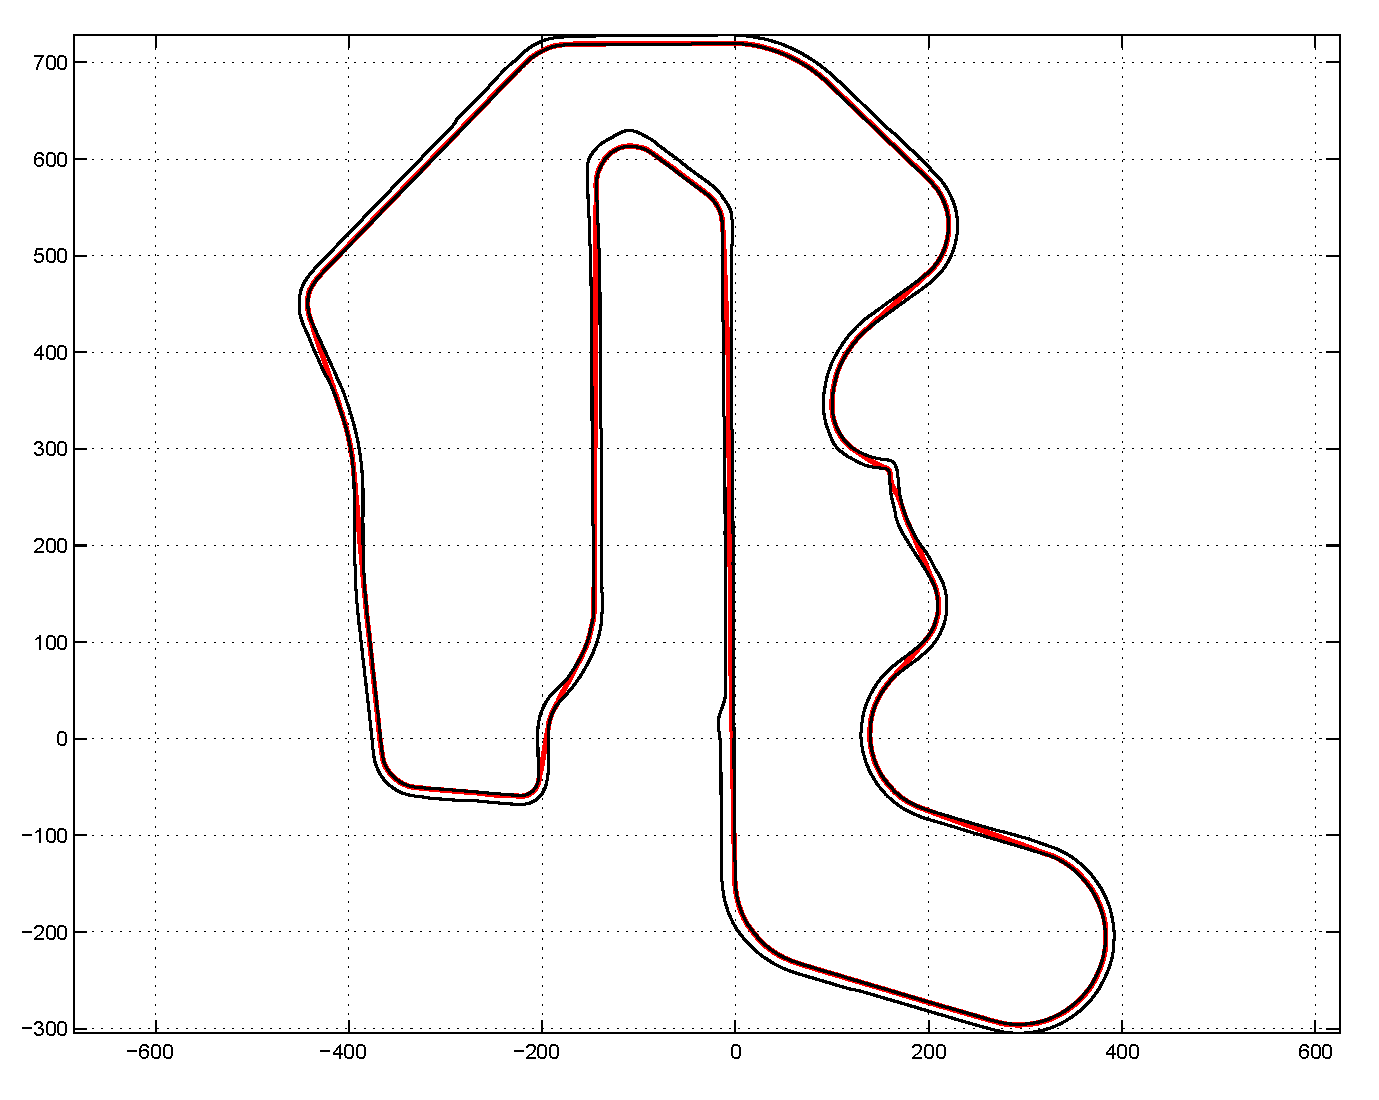
\includegraphics[width=\fullwidth]{shortestpath.eps}
\caption{Minimum distance path around Thunder Hill}
\label{fig:minDist}
\end{figure}

There is clearly a need for a balance between minimizing distance and minimizing curvature, weighted more significantly towards the latter. There have been
several prior attempts in the literature to perform this balance. Braghin \cite{braghin} proposed finding the minimum distance and minimum curvature paths through 
a purely geometric optimization, with no vehicle dynamics considered. Weighted combinations of these
basis paths were then generated and tested using a simple point mass model. For example, let $e_D(s)$ denote the lateral offsets from the track centerline corresponding to the minimum
distance path. Then let $e_\kappa(s)$ be the corresponding offsets for the minimum curvature path. A proposed racing line is then defined by:

\begin{equation}
e = (1-\eta)e_\kappa + \eta e_D
\end{equation}

Where $0 \leq \eta \leq 1$ is the weighting parameter. Figure~\ref{fig:linearCombos} demonstrates this concept for the Thunderhill Racing Circuit. Racing lines generated
with $\eta$ close to 0 are very similar to the minimum curvature path, while candidate solutions with $\eta$ close to 1 approximate the minimum distance path. 

 \begin{figure}
\centering
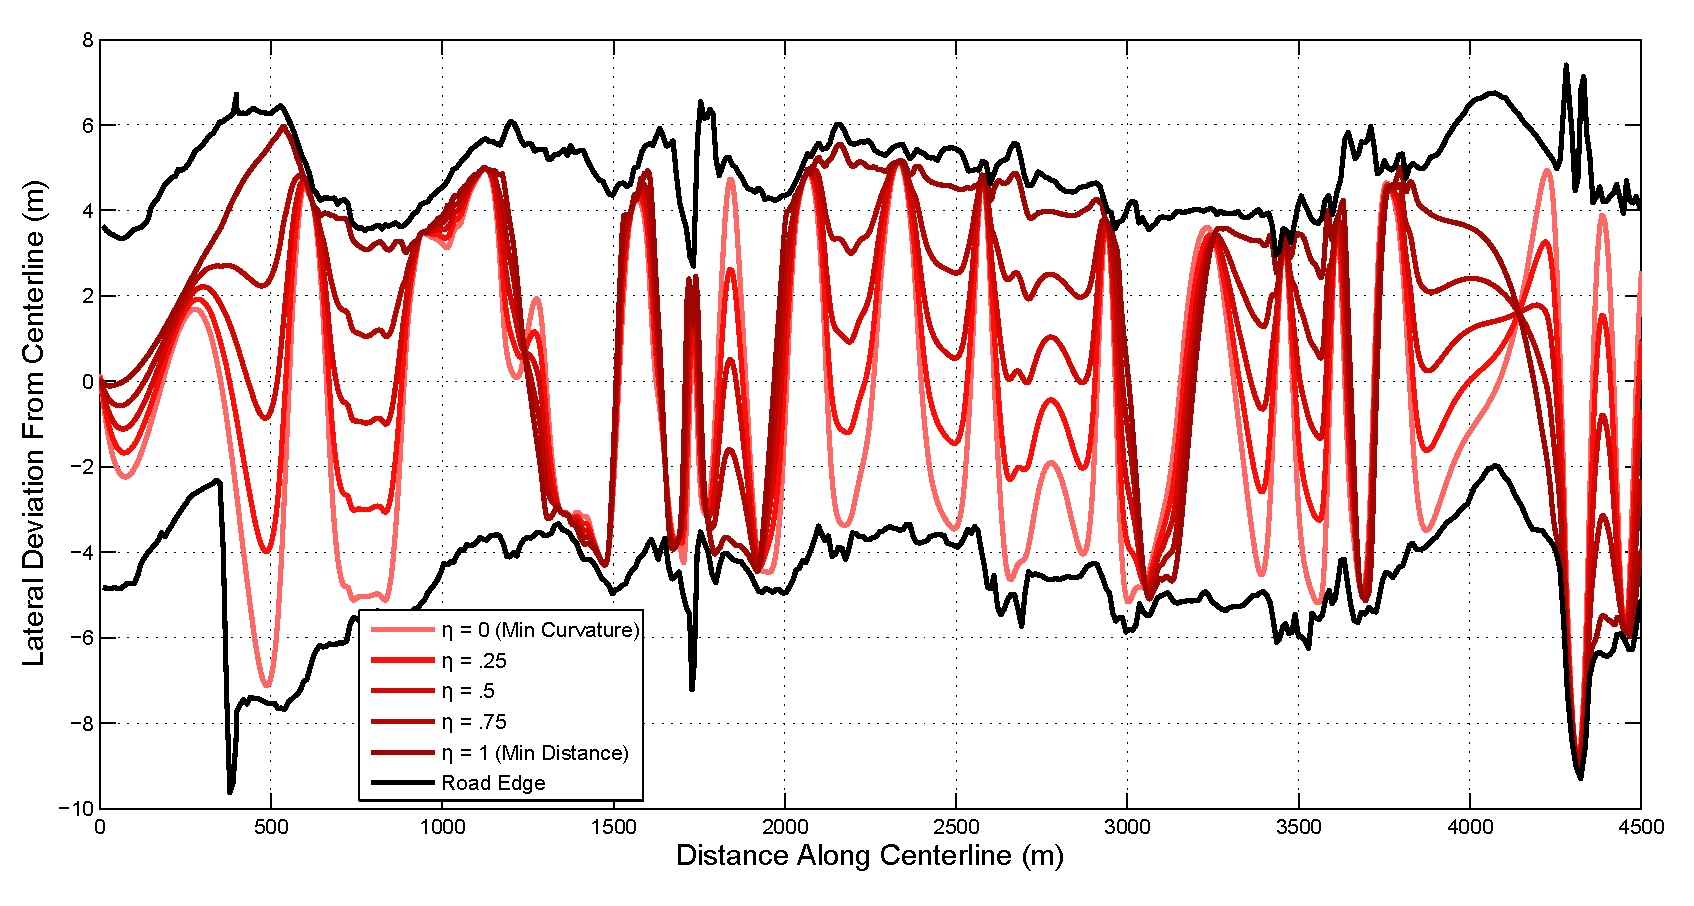
\includegraphics[width=\fullwidth]{linearCombinations.eps}
\caption{A family of racing lines generated from linear combinations of minimum distance and minimum curvature racing lines, with weighting parameter $\eta$.}
\label{fig:linearCombos}
\end{figure}

The issue with this approach is that a single weighting parameter $\eta$ does not adequately balance the tradeoff between minimizing distance and minimizing curvature.
On most sections of a given track, the primary objective is simply to minimize curvature. However, there are typically a small minority of turns (for example, region \circled{c} in our 
case) where minimizing distance traveled is relatively important. A better method is therefore to have the weighting parameter $\eta$ be a function $\eta(s)$ that varies
along the track. This is exactly the approach suggested by Cardamone et al. \cite{cardamone}, who analyzed Braghin's approach over a number of tracks and found that
if only a single weighting factor was chosen, the optimal solution was frequently just $\eta = 0$ (i.e. the minimum curvature path).  

Cardamone et al. suggested determining $\eta(s)$ by applying a genetic algorithm to choose a different weighting parameter between every intersection of the minimum curvature
and minimum distance paths. Similar approaches were also presented by Gadola et al. \cite{gadola} and M{\"u}hlmeier and M{\"u}ller \cite{mully}.
While this provided improved lap times over the minimum curvature solution, genetic algorithms are typically slow computationally, as every candidate solution $\eta(s)$ must be
 simulated. The computational benefit over nonlinear programming that directly minimizes lap time is therefore debatable. 
 
\subsection{Using Human Driver Data to Obtain Optimization \newline Weights}
Using professional driver data as a baseline offers a simpler method to determine parts of the track where minimizing distance is important. Fig.~\ref{fig:DKtrade}(a) shows ten
laps of human driver data on the Thunderhill racetrack overlaid onto Figure~\ref{fig:linearCombos}. Fig.~\ref{fig:DKtrade}(b) shows the resulting weighting
function $\eta(s)$ obtained by averaging the human data and finding the relative distance from the human centerline deviation $e_H(s)$ to the minimum curvature and
minimum distance solutions:

\begin{equation}
\eta(s) = \frac{|e_H(s) - e_\kappa(s)|}{|e_H(s) - e_D(s)|}
\end{equation} 

 \begin{figure}[h!]
\centering
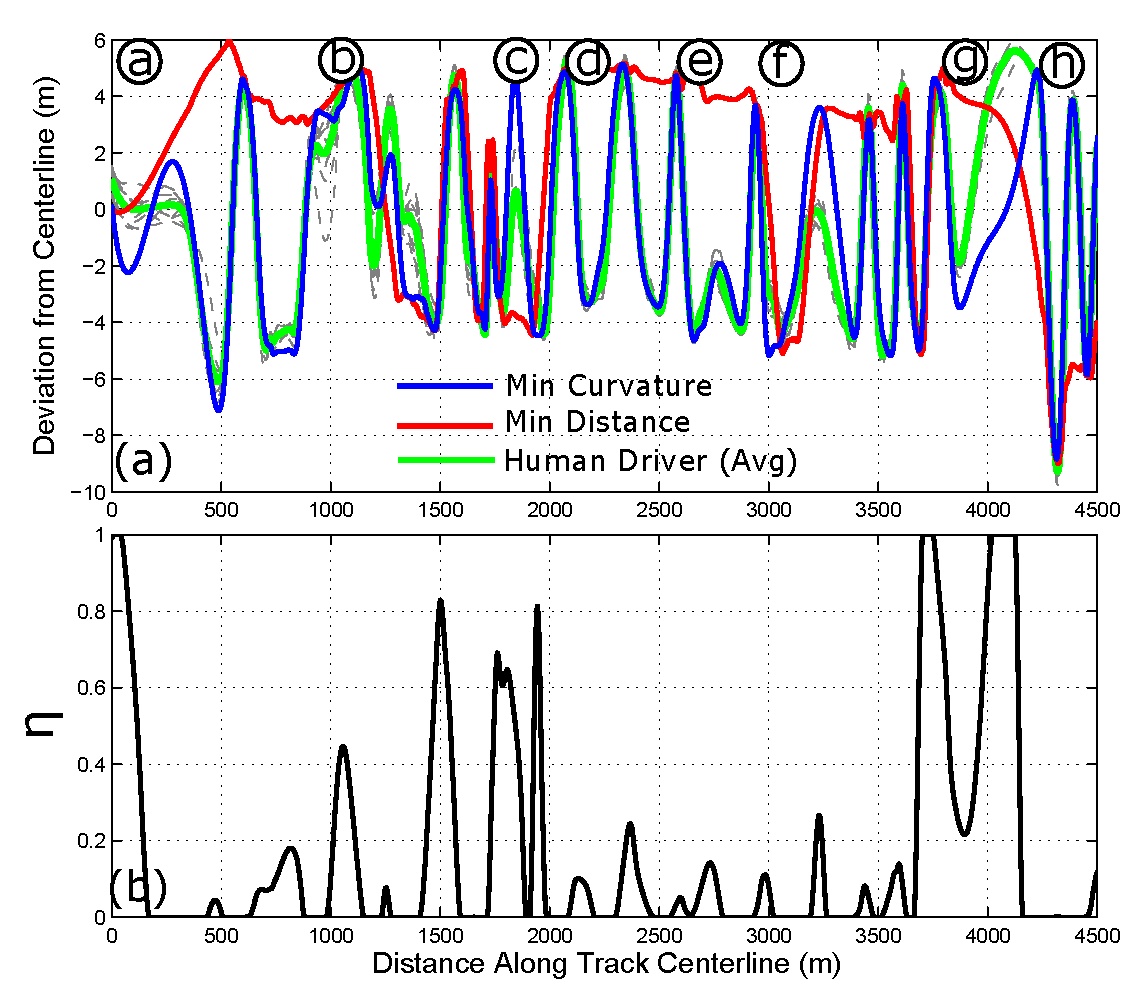
\includegraphics[width=\fullwidth]{distCurvatureTradeoff.eps}
\caption[Ten laps of professional human driver data overlaid over the minimum distance and minimum curvature solutions]{(a) Ten laps of professional human driver data overlaid over the minimum distance and minimum curvature solutions $e_D(s)$ and $e_\kappa(s)$. The average of the human driver
data is shown in green, and the individual datasets are shown in light grey. (b) Values of $\eta(s)$ from human data, with low pass filter applied to eliminate rapid changes. Values are also limited to range from 0 to 1.}
\label{fig:DKtrade}
\end{figure}

\newpage
This definition is only relevant if the human racing line is bounded by the minimum distance and minimum curvature racing lines. Since this is frequently not
the case in Fig.~\ref{fig:DKtrade}(a), $\eta(s)$ is set to 1 if $e_H(s) < e_D(s) < e_\kappa(s)$ or 0 if $e_H(s) < e_\kappa(s) < e_D(s)$. Furthermore, a low-pass filter is also applied to Fig.~\ref{fig:DKtrade}(a) to eliminate rapid changes in $\eta(s)$.

Fig.~\ref{fig:DKtrade} shows that there are several regions of the track where the human drives closer to to the minimum distance racing line (i.e. locations where
$\eta$ is significantly greater than 0). Most of these are trivial, occurring in locations where the minimum distance and minimum curvature racing lines are
relatively close. However, in region \circled{c}, the professional human driver is on average about halfway between the minimum distance and minimum curvature solutions,
an interesting result. Furthermore, on straight sections of the track such as \circled{a} and \circled{g}, the human driver appears to be seeking a minimum distance path as well. 

\subsection{Combined Cost Function and Simulated Results}

Using the information from Fig.~\ref{fig:DKtrade}, the combined cost function for the path update step in (\ref{eq:OPT}) is given by:

\begin{equation}
\label{eq:OPT2}
\underset{\delta, \hspace{.5mm} e, \hspace{.5mm} \Psi, \hspace{.5mm} \Delta\Psi, \hspace{.5mm} \beta}{\text{minimize}} \quad \sum_{k} \left(\frac{\Psi_k - \Psi_{k-1}}{s_k - s_{k-1}}\right)^2 + \lambda\sum_k \frac{\eta_k \Delta s_k}{U_{xk}} \left(-\kappa_ke_k + (\Delta\Psi_k + \beta_k)^2\right)
\end{equation}

The first summation in (\ref{eq:OPT2}) is the same curvature minimization term, while the second summation represents the distance minimization term. The weights
$\eta_k$ from Fig.~\ref{fig:DKtrade}(a) are used to determine how much of the minimum distance term to use at each point along the track. This approach is fundamentally
different from the methods in \cite{braghin} and \cite{cardamone}. The prior approaches search a space of solutions to find the best linear combination of the \textit{pre-calculated} minimum distance and minimum curvature racing
lines, with weights given by a constant $\eta$ or function $\eta(s)$. The presented approach performs a single optimization for each path update step, with the \textit{optimization weights} given by $\eta_k$. As a result, there is 
an additional tunable parameter $\lambda$ in (\ref{eq:OPT2}) with units of seconds, that ensures units of both summation terms are the same.

There are several benefits of the proposed approach. First, since we obtained $\eta(s)$ from human driver data, simply applying a linear combination with weights $\eta(s)$ would
trivially give back the averaged professional driver's racing line. More importantly, however, using pure linear combinations of two precomputed solutions provides excessive restrictions on the resulting racing lines. 
This is because the resulting solutions can never explore regions that are not contained within the minimum curvature and minimum distance solutions. Furthermore, there is no guarantee the resulting path will be experimentally drivable. 
Even if the minimum curvature and distance paths come from an optimization with vehicle dynamics constraints, if the weighting function $\eta(s)$ is not sufficiently smooth, there will be discontinuities in
the resulting curvature profile. By using $\eta(s)$ to instead guide the optimization, the resulting curvature profile will always be smooth. 


 \begin{figure}
\centering
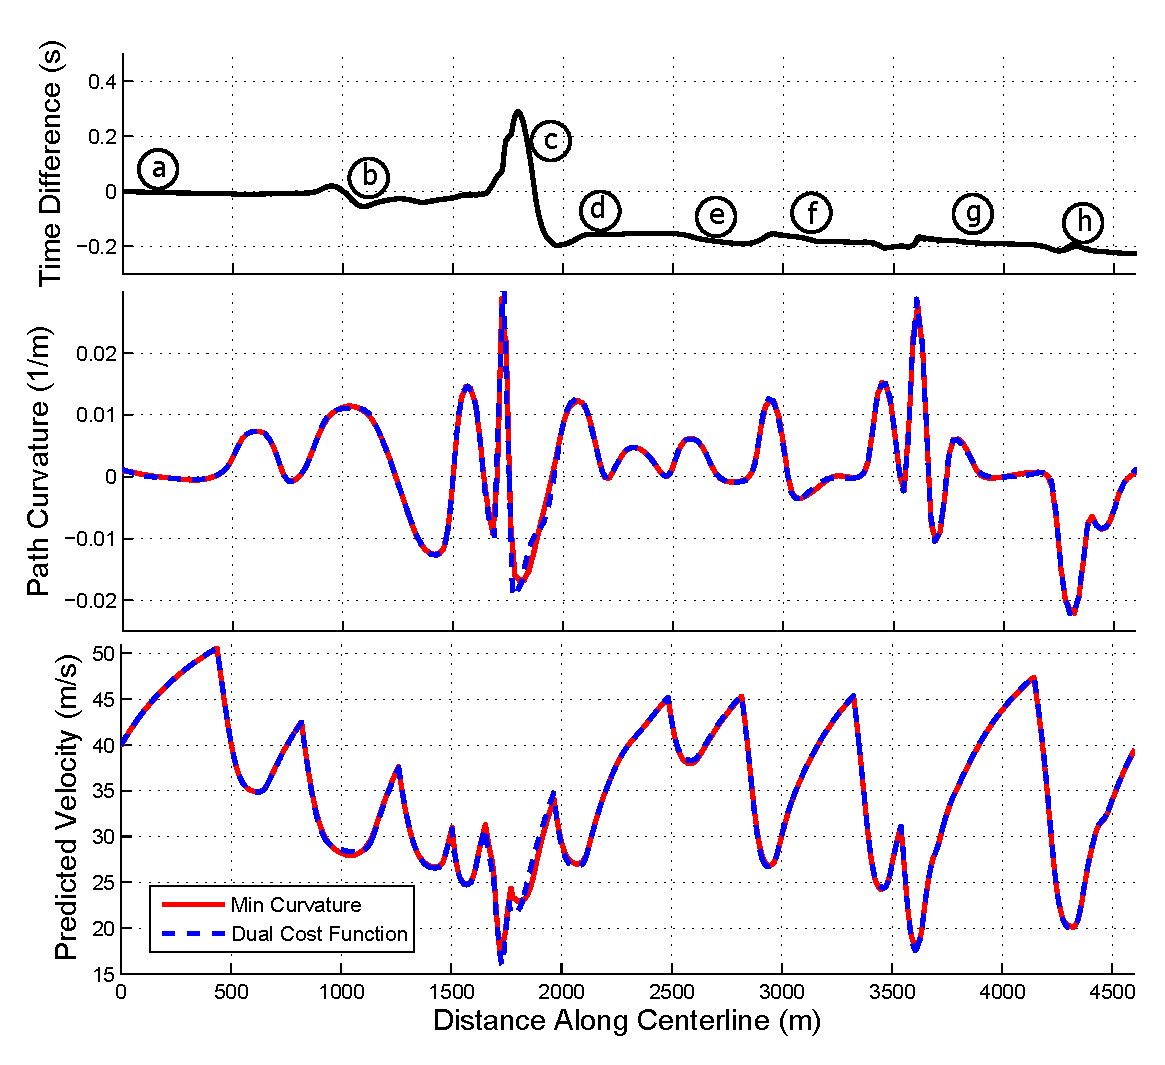
\includegraphics[width=\fullwidth]{simWithMinDist.eps}
\caption[Simulation results comparing minimum curvature cost function with weighted cost function]{Simulation results comparing minimum curvature cost function with weighted distance/curvature cost function ($\lambda = 0.05$ sec). (a) Time difference between two solutions as a function
of distance along centerline, with a negative time
difference corresponding to the weighted optimization being ahead. (b) Path curvature. (c) Simulated velocities.}
\label{fig:SD2}
\end{figure}

Fig.~\ref{fig:SD2} shows simulation results when the fast generation method is run for five iterations. The simulation compares the racing lines
 generated by the curvature minimization cost function and the combined curvature-distance cost functions. 
Unsurprisingly, the primary difference occurs at region \circled{c}. With the combined cost function, the resulting racing line takes a slightly higher curvature turn on the initial left turn. While this
initially loses time, the resulting solution can minimize distance traveled on the next turn, resulting in an overall time advantage of 0.2 seconds. 

 \begin{figure}
\centering
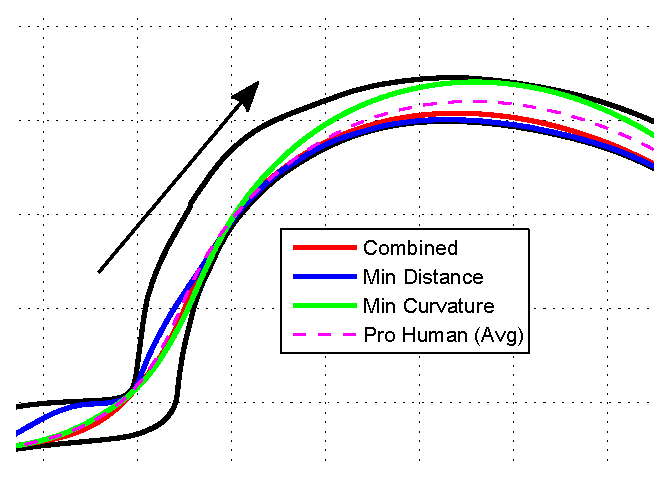
\includegraphics[width=.7\fullwidth]{regC.eps}
\caption[Racing lines for minimum curvature, minimum distance, and combined cost functions around region c.]{Racing lines for minimum curvature, minimum distance, and combined cost functions around region c. Notice that with the combined cost function,
the resulting racing line is not bounded by the minimum curvature and minimum distance solutions. Averaged pro human racing line is shown as well.}
\label{fig:regC}
\end{figure}

The minimum distance,
minimum curvature, and combined racing lines at region \circled{c} are shown in Fig.~\ref{fig:regC}. The combined solution follows the minimum curvature solution more
closely for the initial left-hand turn, but the minimum distance solution more closely for the second right-hand turn. Additionally, the racing line
from the dual cost function is not always inside the minimum distance and minimum curvature racing lines. This demonstrates the advantage of a weighted cost function
as opposed to a linear combination of pre-calculated solutions.  

\section{Discussion and Future Work}
\label{sec:DISCUSSION}

The primary benefit of the proposed algorithm is not improved lap time performance
over the nonlinear algorithm but rather a radical improvement in computational simplicity and speed. Each two-step iteration of the full
course takes only 26 seconds on an Intel i7 processor, whereas the nonlinear algorithm from \cite{theodosis} typically runs over the course of several hours on the same
machine. The most significant computational expense for the proposed algorithm is solving the convex curvature minimization problem for
all 1843 discrete time steps $T$ over the 4.5 km racing circuit.

\begin{table}[h]
\begin{center}
\caption{Iteration Computation Time}\label{tb:solvetime}
\begin{tabular}{ccc}
Lookahead (m) & $T$ & Solve Time (s) \\\hline
450& 184 &5 \\
900&  369 & 6 \\
1800& 737 & 12 \\
4500& 1843& 26 \\\hline
\end{tabular}
\end{center}
\end{table}

This computational efficiency will enable future work to incorporate the trajectory modification algorithm as an online
 ``preview" path planner, which would provide the desired vehicle trajectory for an upcoming portion of the race track. 
 Since the computation time of the algorithm is dependent on the preview distance, 
 the high-level planner would not need to run at the same sample time as the vehicle controller. Instead, the planner would operate on a separate CPU and provide a velocity profile and racing line for only
 the next 1-2 kilometers of the race track every few seconds, or plan a path for the next several hundred meters within a second.
 
 Table \ref{tb:solvetime} shows problem solve times for a varying range of lookahead lengths with the same discretization $\Delta s$,
 and shows that the runtime scales roughly linearly with the lookahead distance. The above solve times are listed using the CVX convex optimization solver, which 
 is designed for ease of use and is not optimized for embedded computing. Preliminary work has been successful
 in implementing the iterative two-step algorithm into C code using the CVXGEN software tool \cite{boydcvxgen}. When written
 in optimized C code, the algorithm can solve the curvature minimization problem (\ref{eq:OPT}) in less than 0.005 seconds for a lookahead distance of 650 meters.
 
 The possibility of real-time trajectory planning for race vehicles creates several fascinating areas of future research. An automobile's surroundings are subject to both rapid and
 gradual changes over time, and adapting to unpredictable events requires an approximate real-time trajectory planning algorithm.
 On a short time scale, the real-time trajectory planner could find a fast but stable recovery trajectory in the event of the race vehicle entering an understeer or oversteer 
 situation. On an intermediate time scale, the fast executing two-step algorithm could continuously plan a racing line in the presence of other moving race vehicles by constraining the
 permissible driving areas to be collision-free convex ``tubes" \cite{erlien}.  Finally, the algorithm could update the trajectory given estimates of the friction coefficient and other vehicle parameters learned gradually over
 time.
 
\section{Conclusion}
This chapter demonstrates an iterative algorithm for quickly generating vehicle racing trajectories, where each iteration is comprised of
 a sequential velocity update and path update step. Given an initial path through the race track, the 
 velocity update step performs forward-backward integration to determine the minimum-time speed inputs. Holding this speed 
 profile constant, the path geometry is updated by solving a convex optimization problem to minimize path curvature.

 The primary benefit of the presented trajectory planner is computational speed. Experimental data on an autonomous race vehicle over a
 three mile race course confirms that the trajectory generated by the algorithm provide comparable lap times to that from a nonlinear gradient descent algorithm. However, the
 required computation time is at least two orders of magnitude faster. One drawback of the presented approach is that lap time is not explicitly minimized, resulting
 in sub-optimal performance on complex sequences of turns. A second analysis was therefore conducted in simulation to show the
 benefit of adding a distance minimizing term to the convex path update step. An exciting opportunity for future research is incorporating the trajectory modification algorithm into an online path planner to provide
 racing trajectories in real time. 
 
 \textit{Note: This chapter reuses material previously published by the author in \cite{kapaniadscc}.}
